\section{Evaluation}
\label{sec:result}
\begin{figure*}[htb]
    \centering
    \begin{minipage}{0.32\linewidth} %full res
        \subfloat[gas scene(\textbf{GT})]{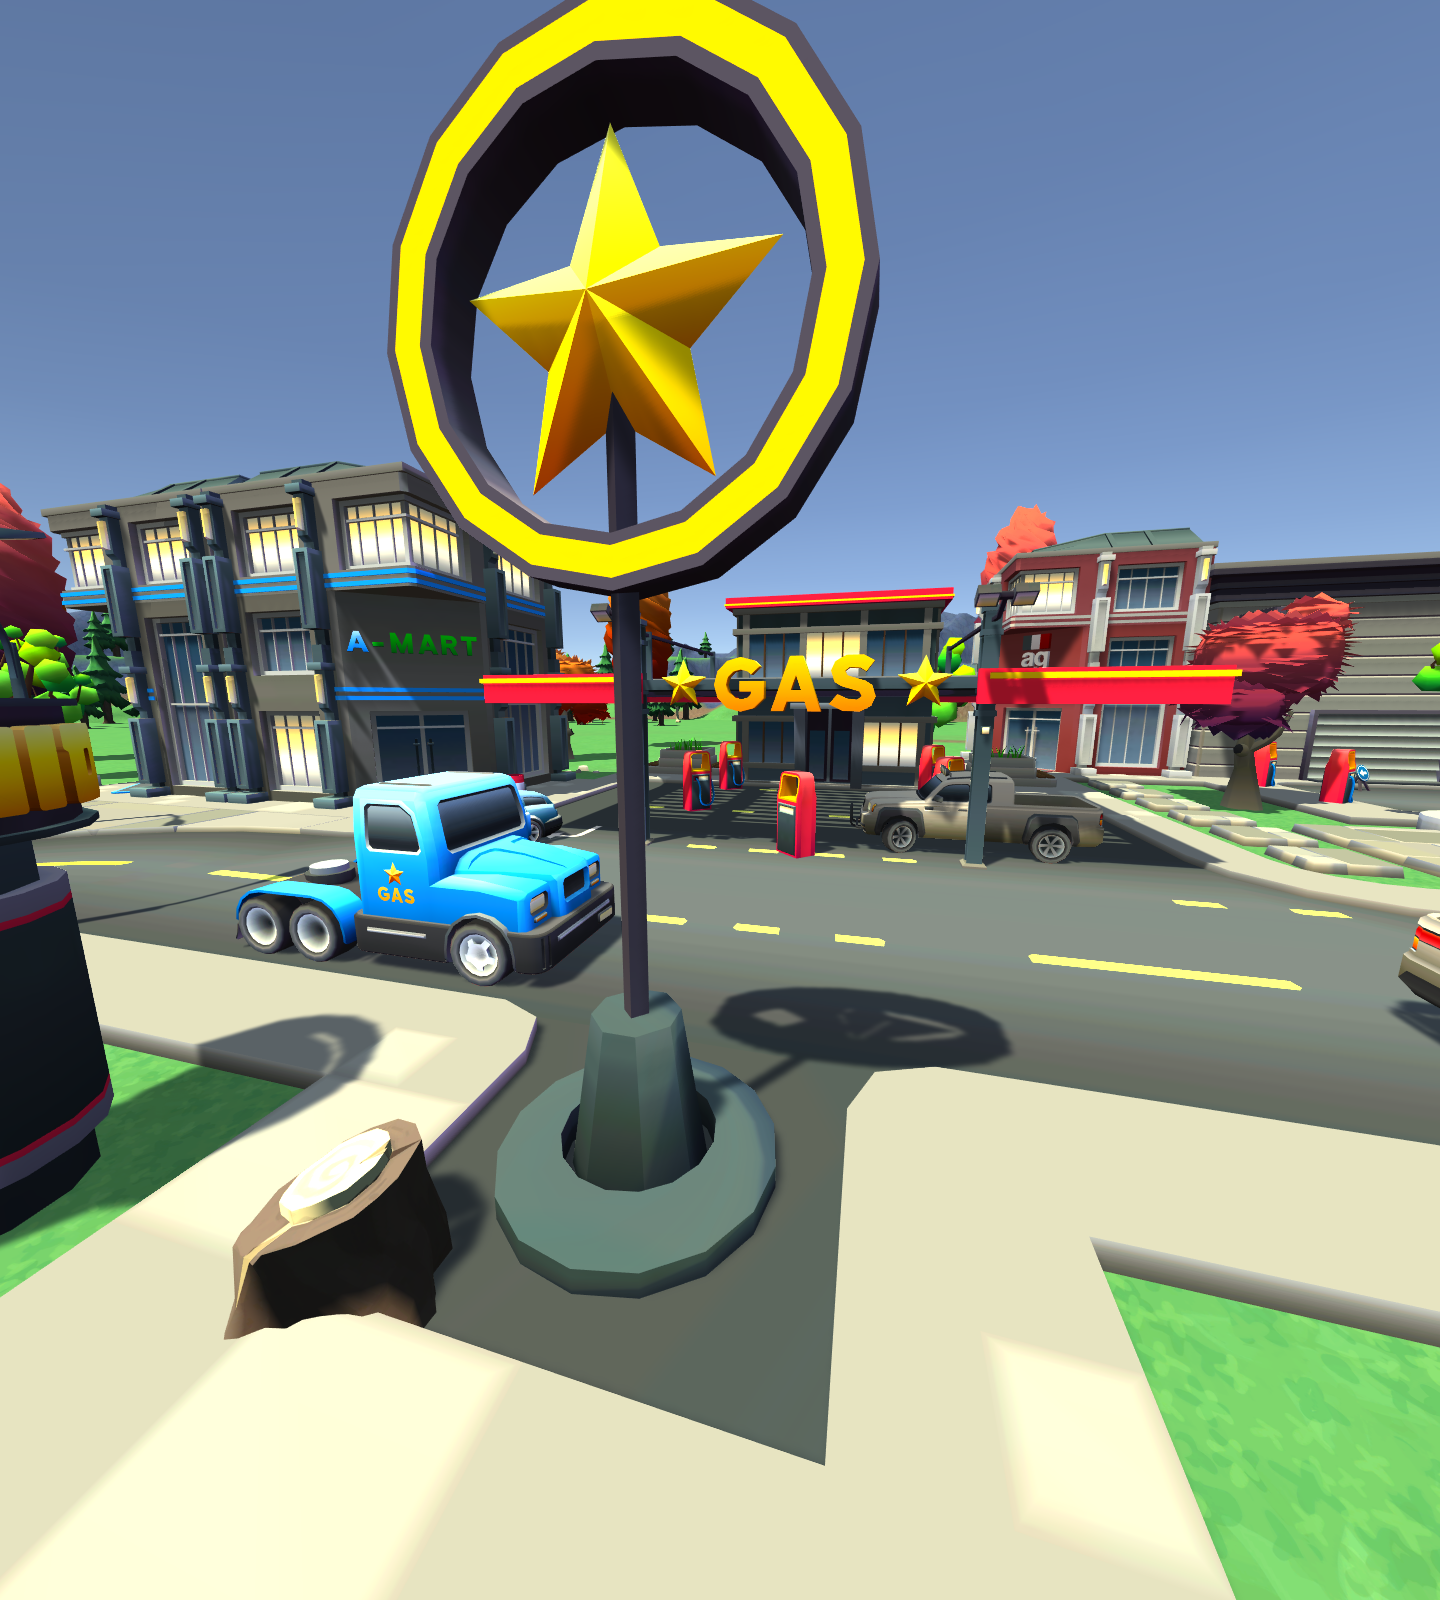
\includegraphics[width=0.96\linewidth]{TOG/figs/gas_gt4.png}}
        
        \subfloat[minecraft scene(\textbf{GT})]{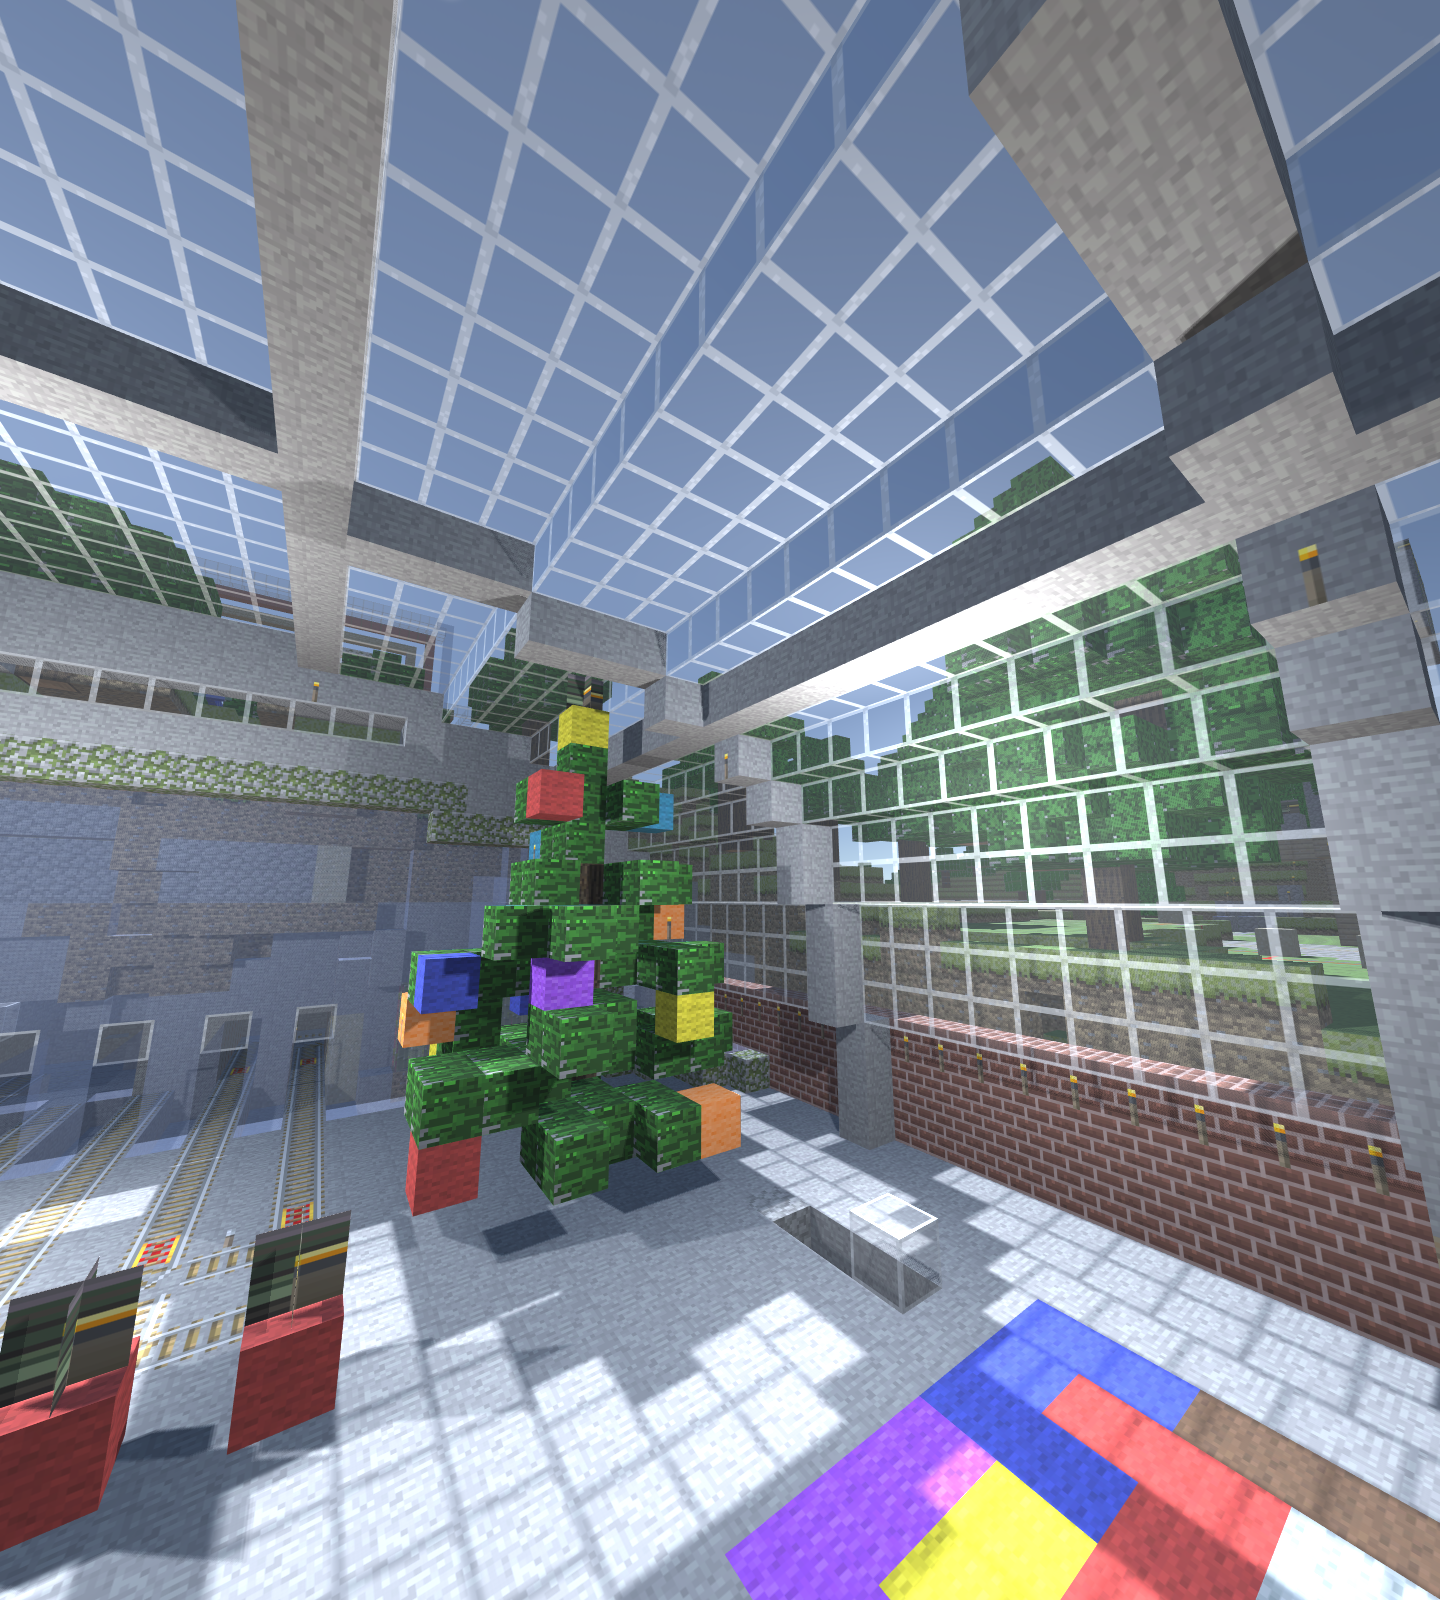
\includegraphics[width=0.96\linewidth]{TOG/figs/mc_gt3.png}}
        
        \subfloat[bedroom scene(\textbf{GT})]{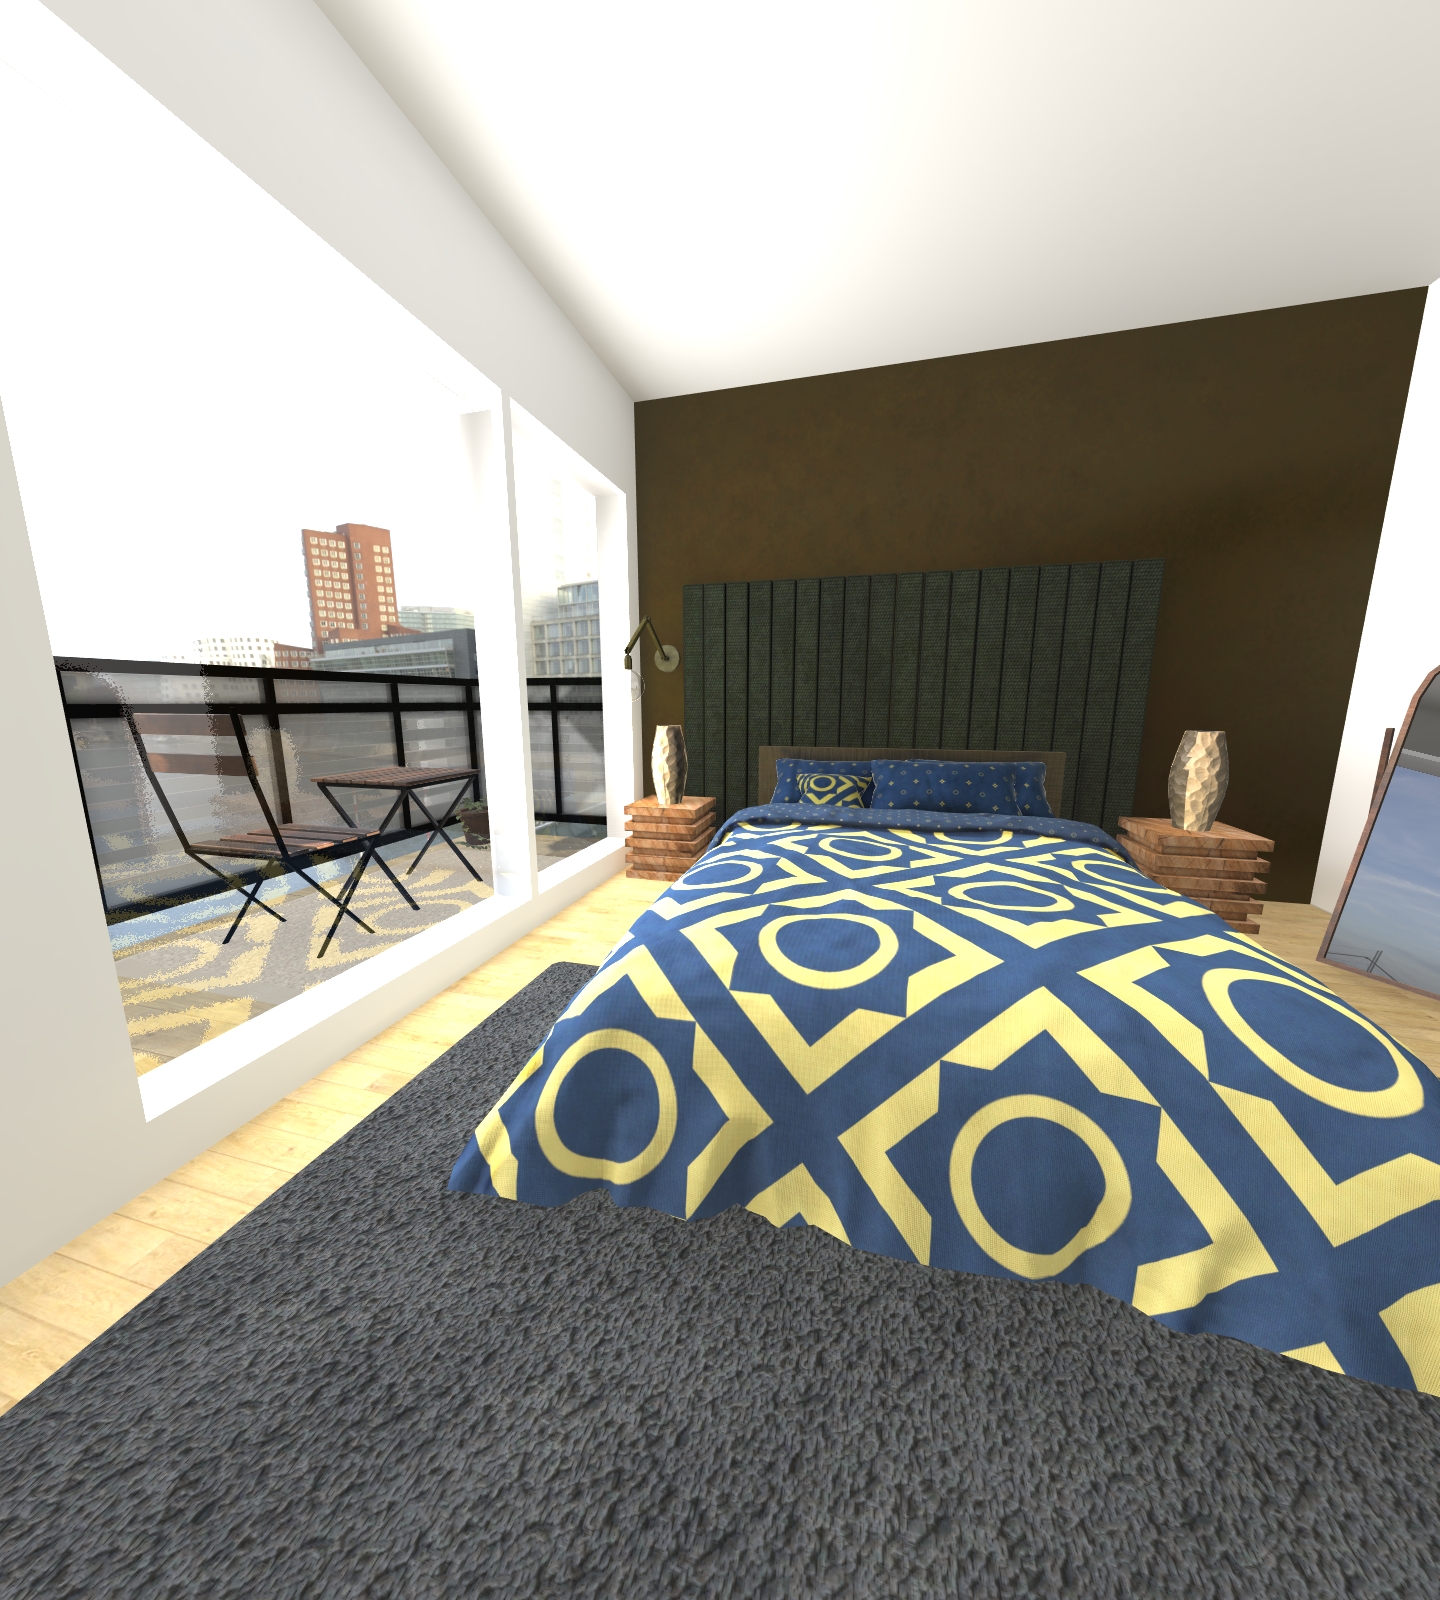
\includegraphics[width=0.96\linewidth]{TOG/figs/bed_gt0.png}}
    \end{minipage}
    \begin{minipage}{0.32\linewidth} %ours
        \subfloat[gas scene (\textbf{OUR})]{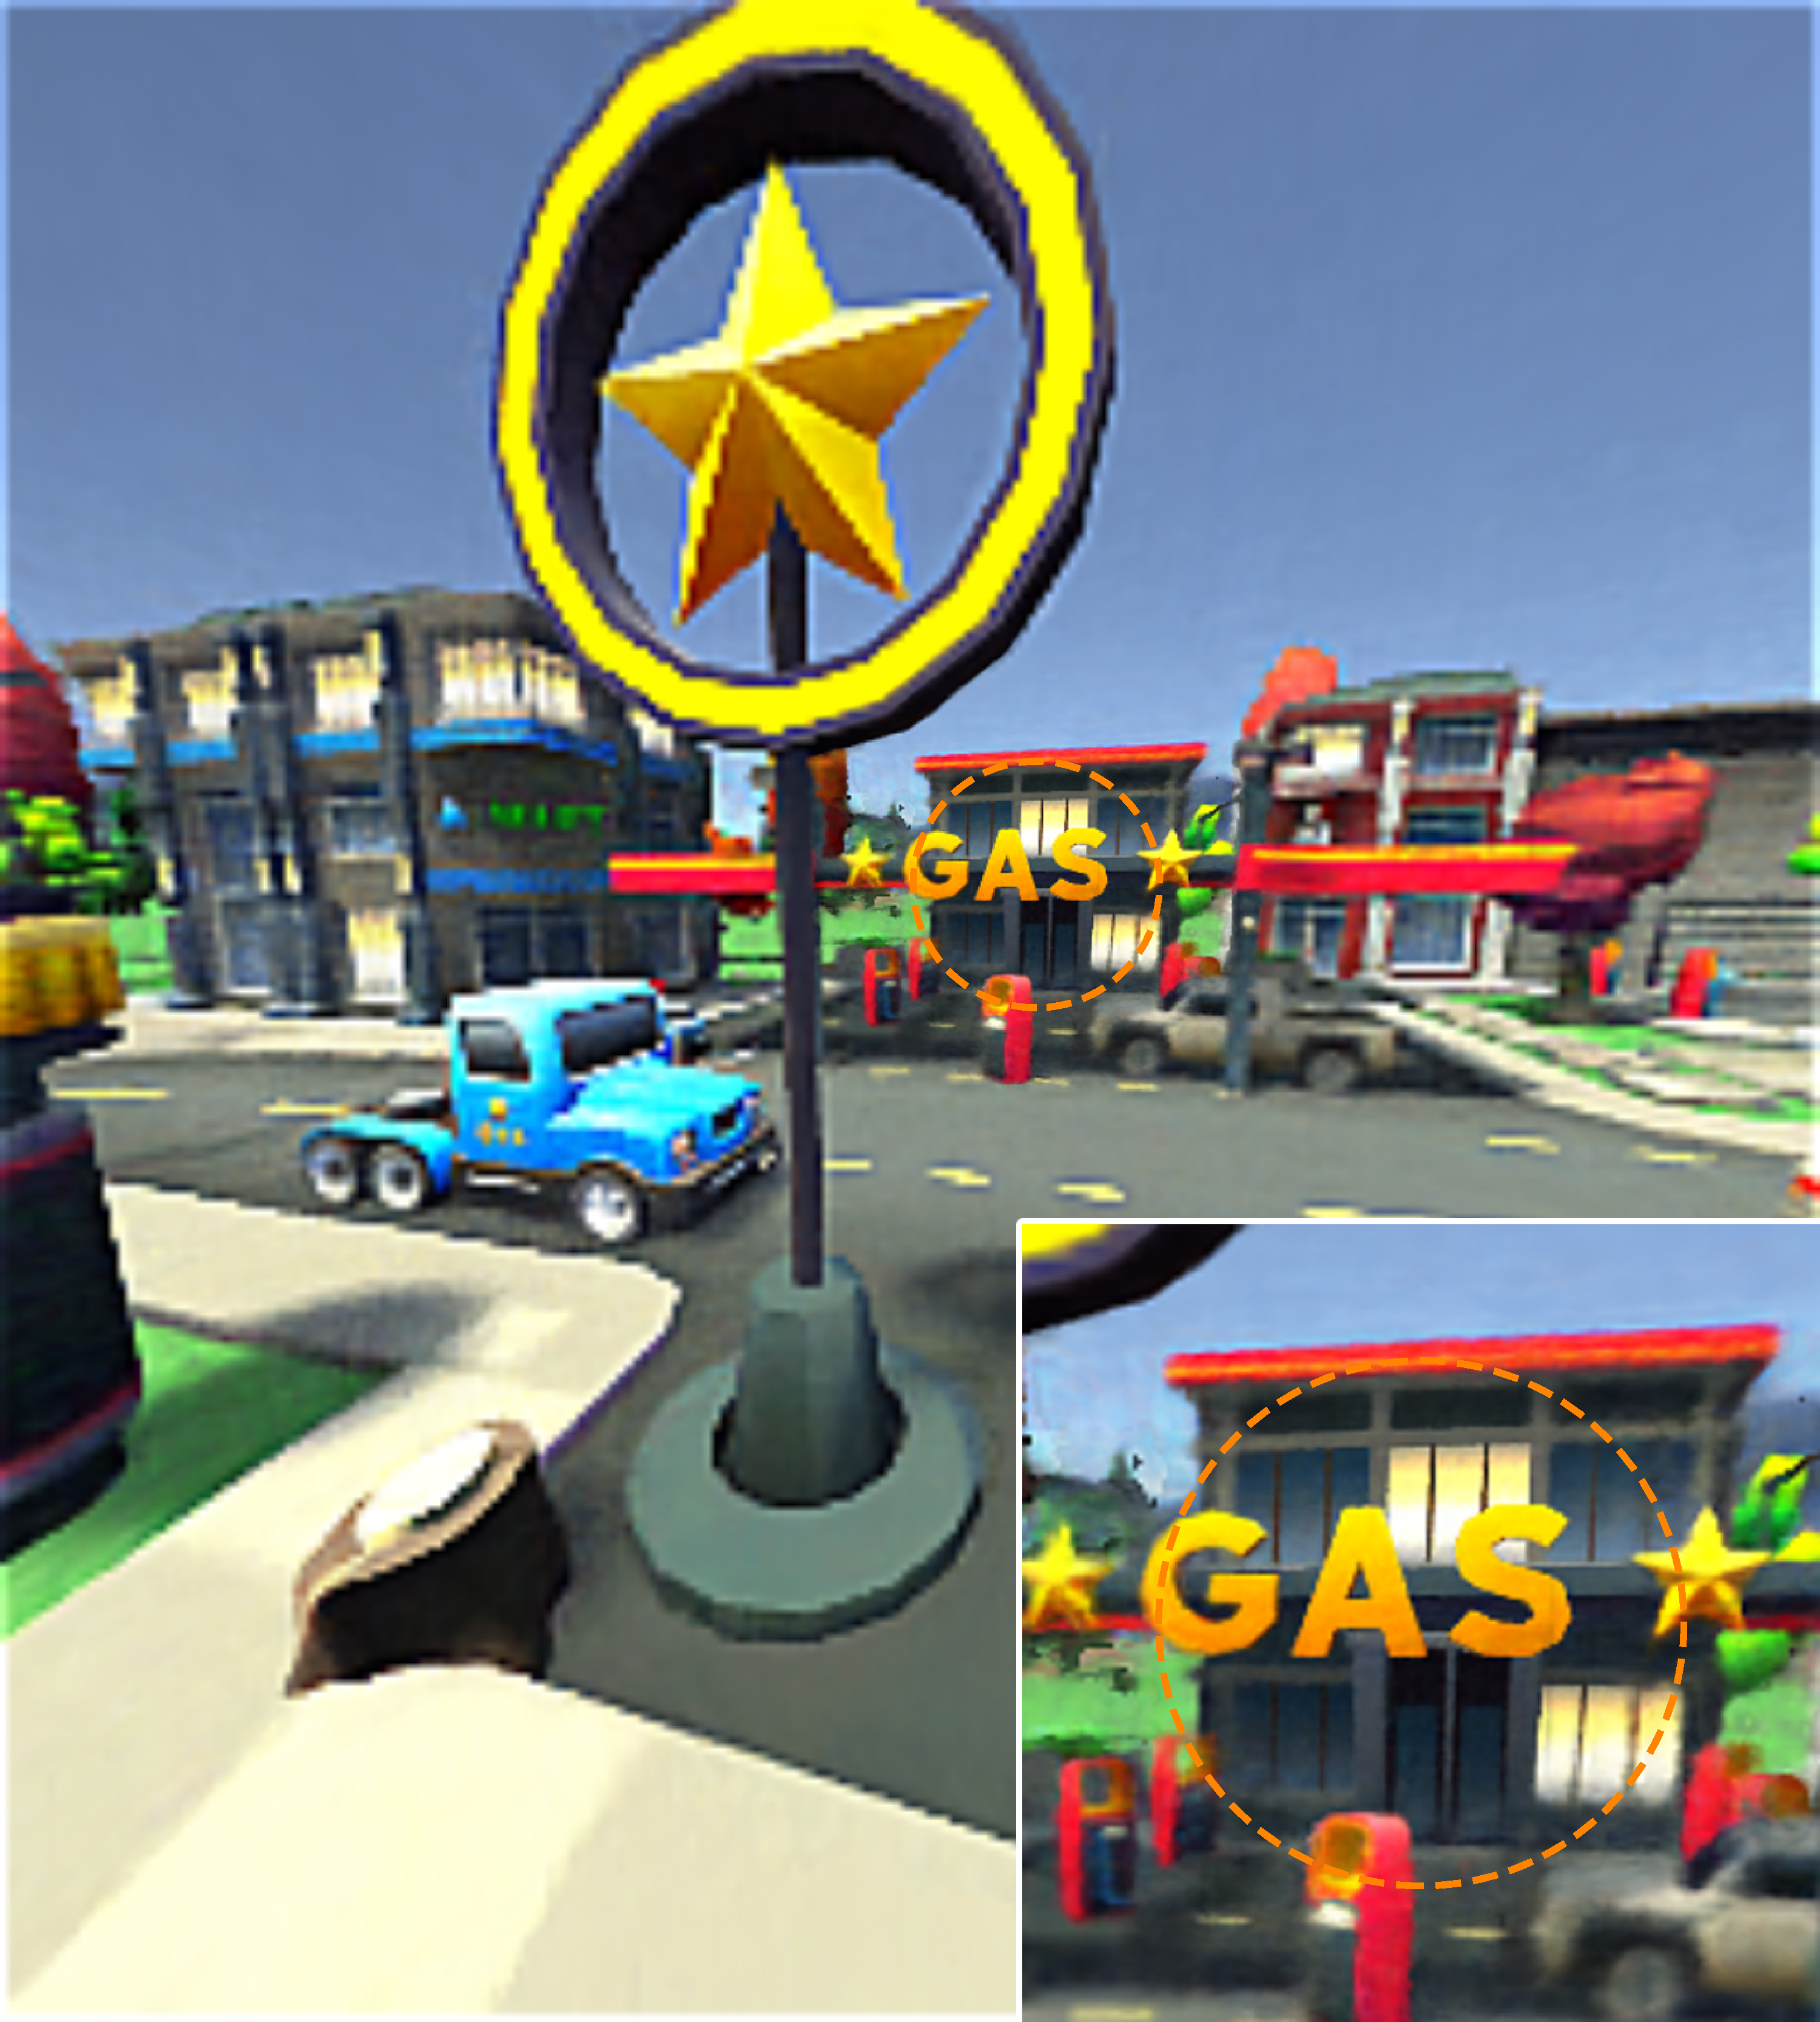
\includegraphics[width=0.96\linewidth]{TOG/figs/gas_our4_inset.pdf}}
        
        \subfloat[minecraft scene (\textbf{OUR})]{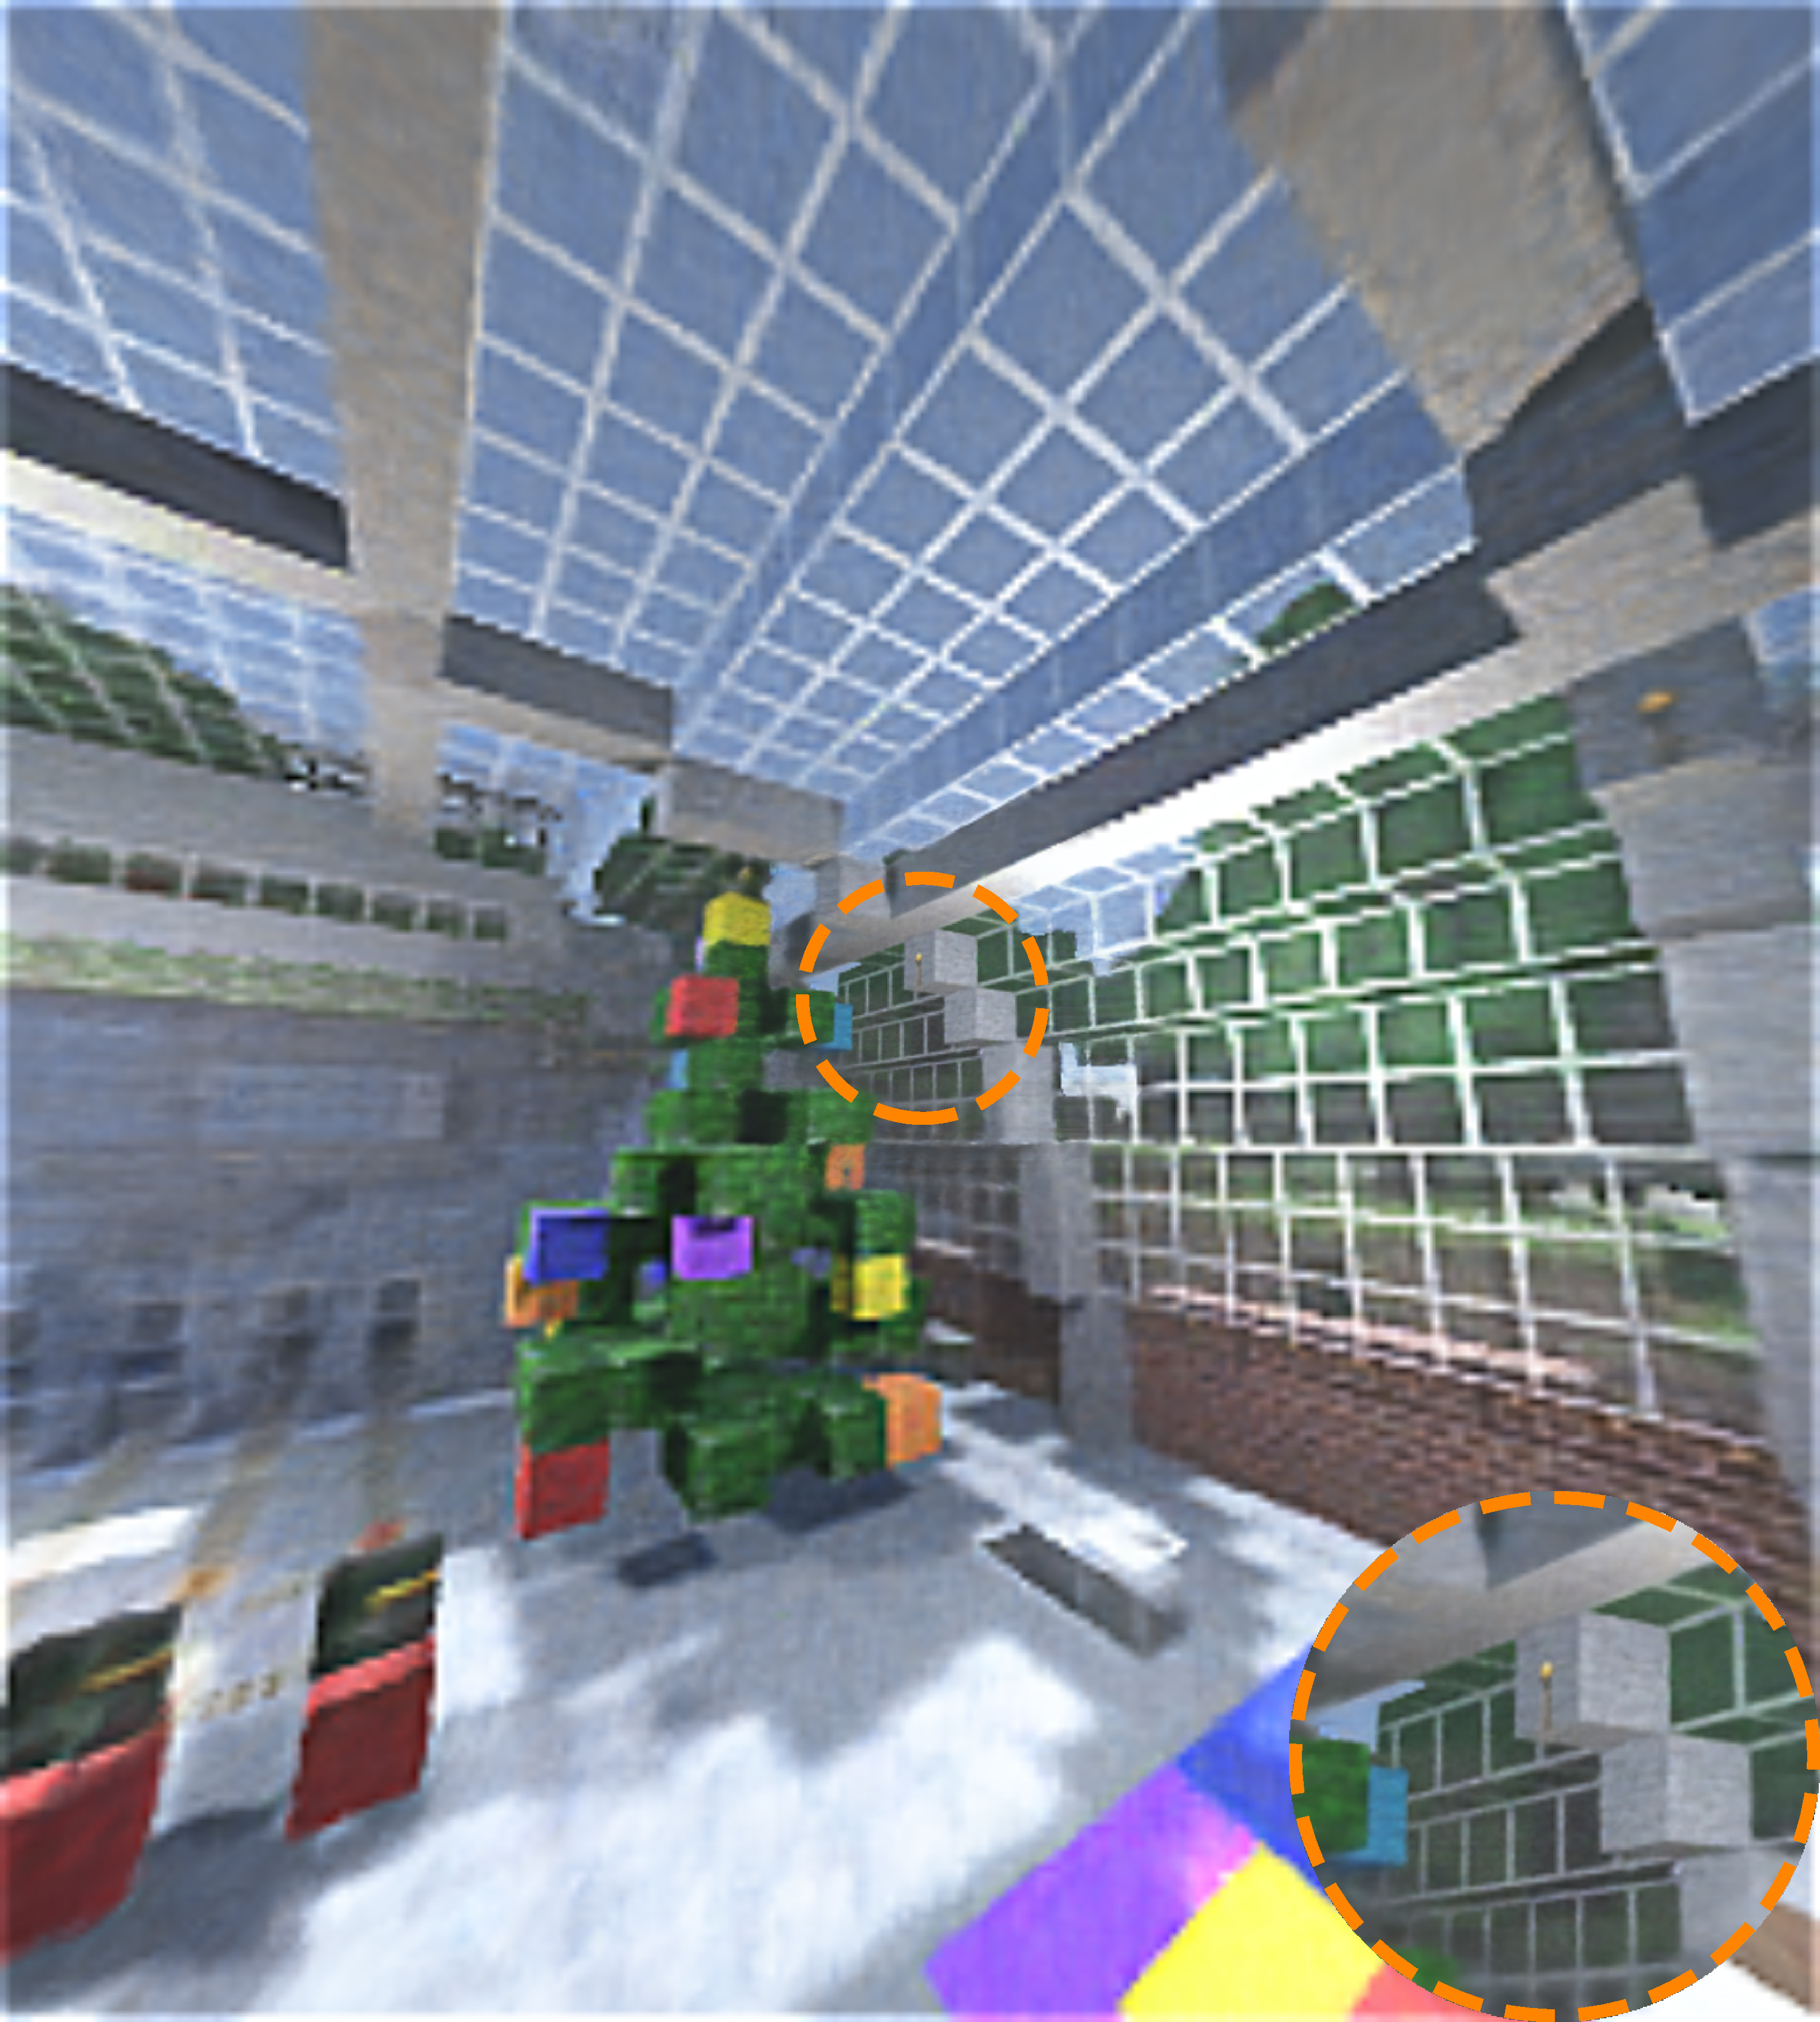
\includegraphics[width=0.96\linewidth]{TOG/figs/mc_our3_inset.pdf}}
        
        \subfloat[bedroom scene (\textbf{OUR})]{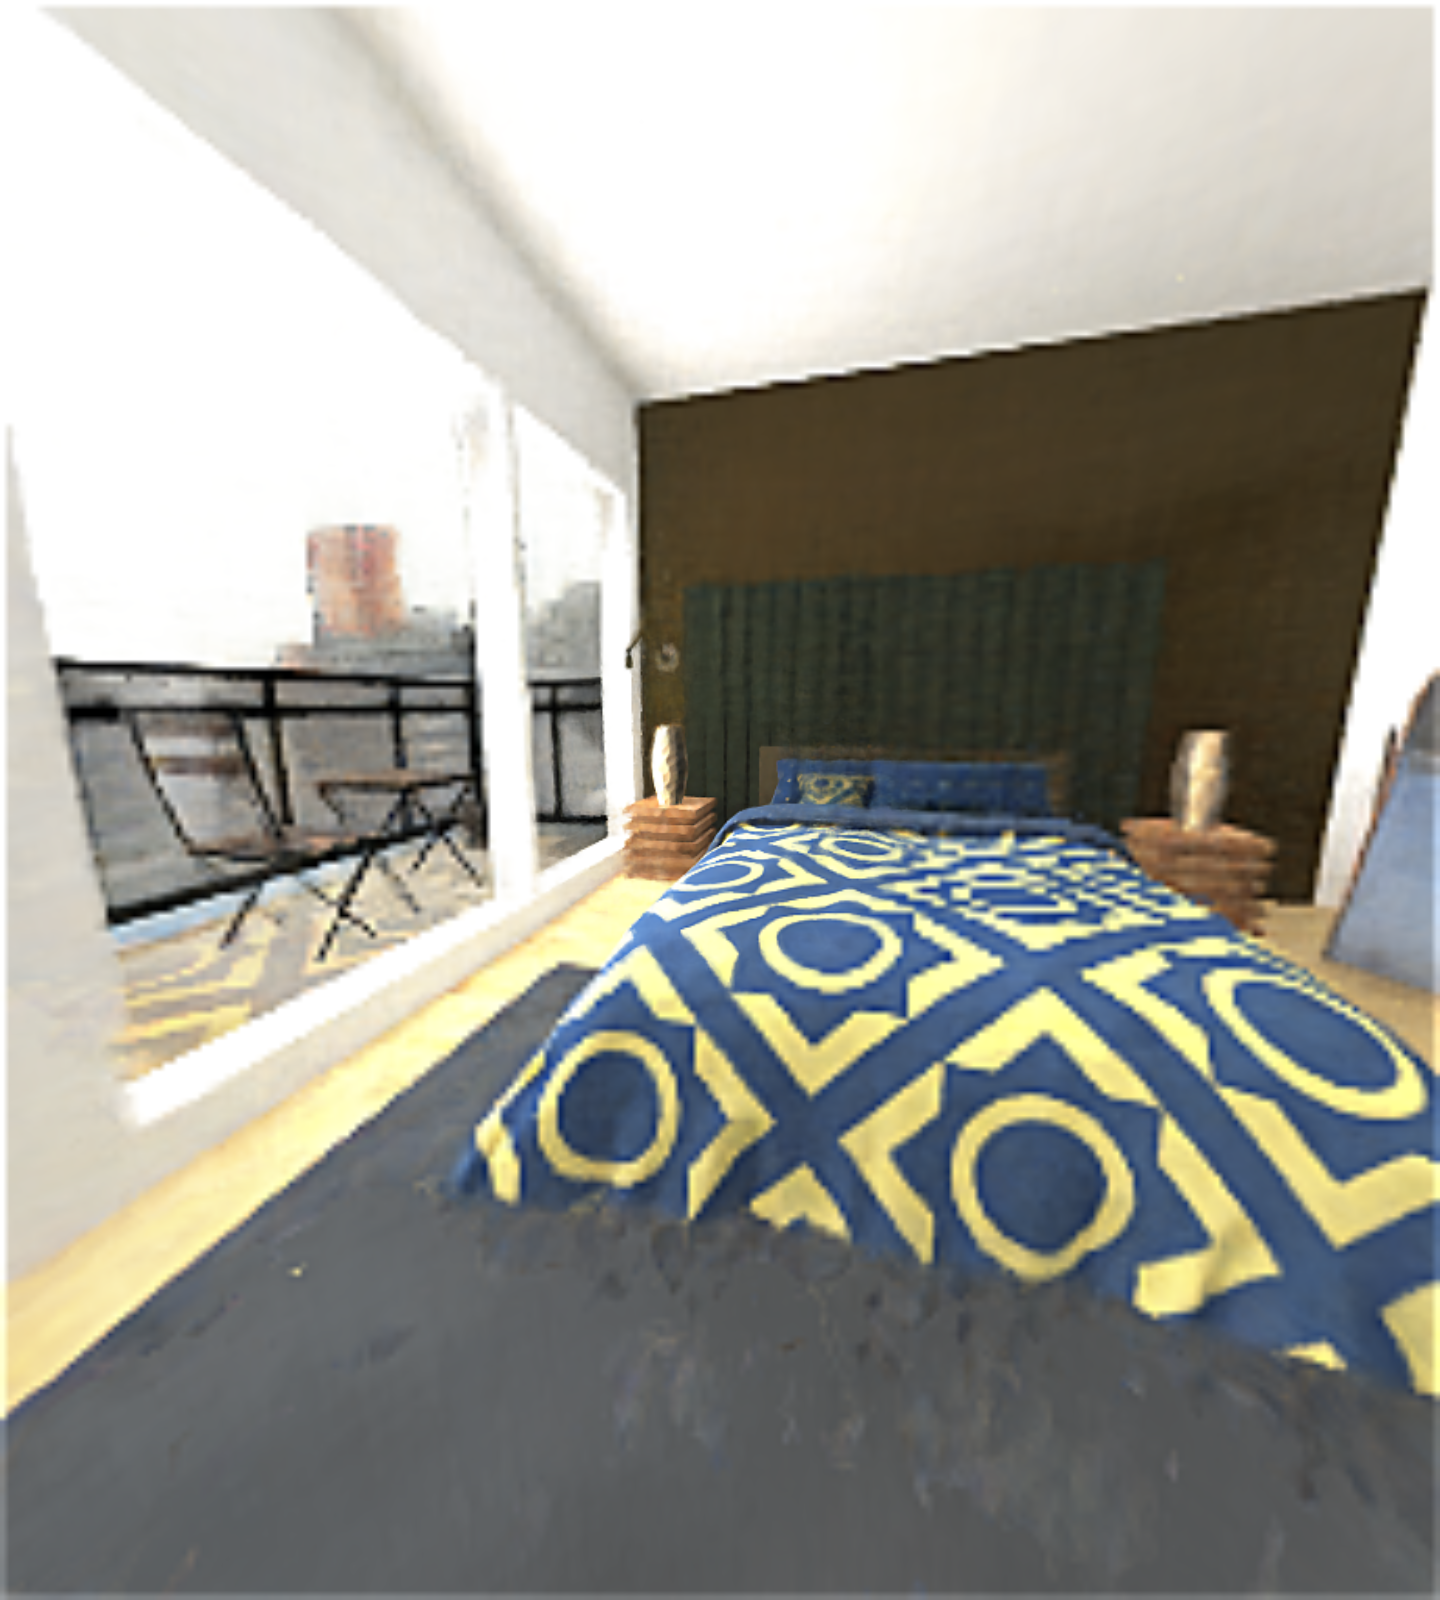
\includegraphics[width=0.96\linewidth]{TOG/figs/bed_our0.png}}               
    \end{minipage}
    \begin{minipage}{0.32\linewidth} % NERF
        \subfloat[gas scene (\textbf{NeRF})]{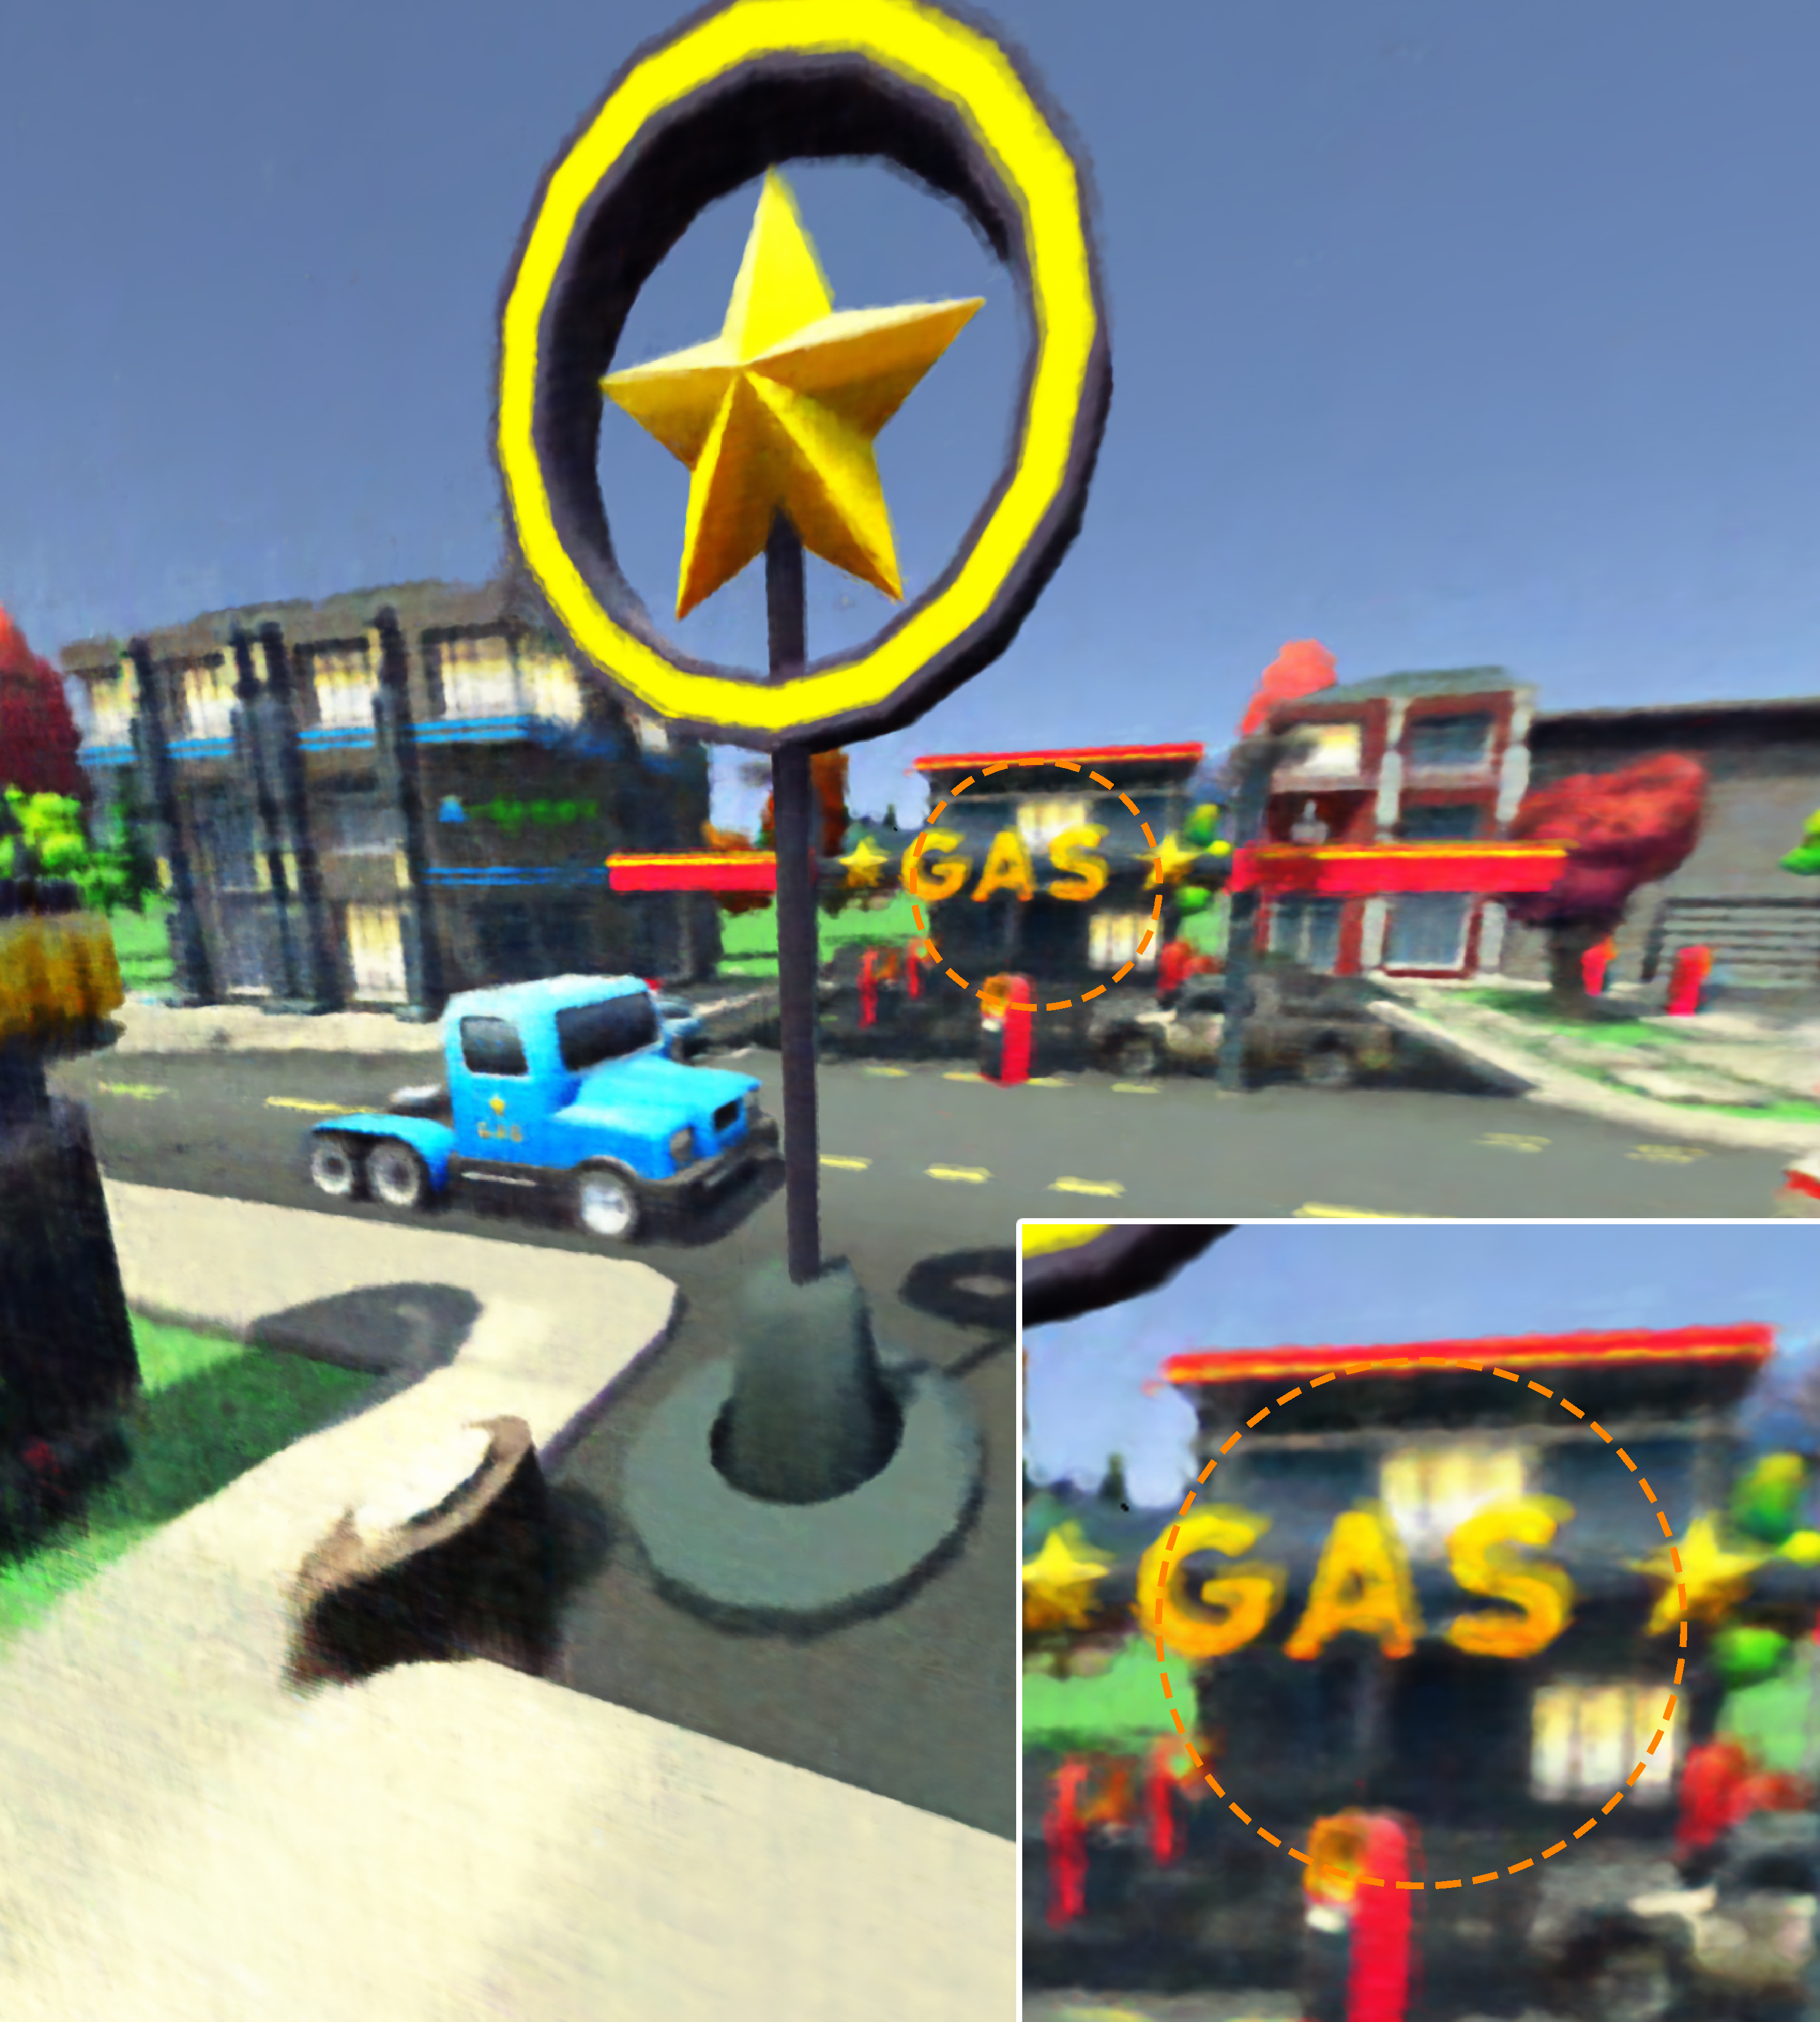
\includegraphics[width=0.96\linewidth]{TOG/figs/gas_nerf4_inset.pdf}}
        
        \subfloat[minecraft scene (\textbf{NeRF})]{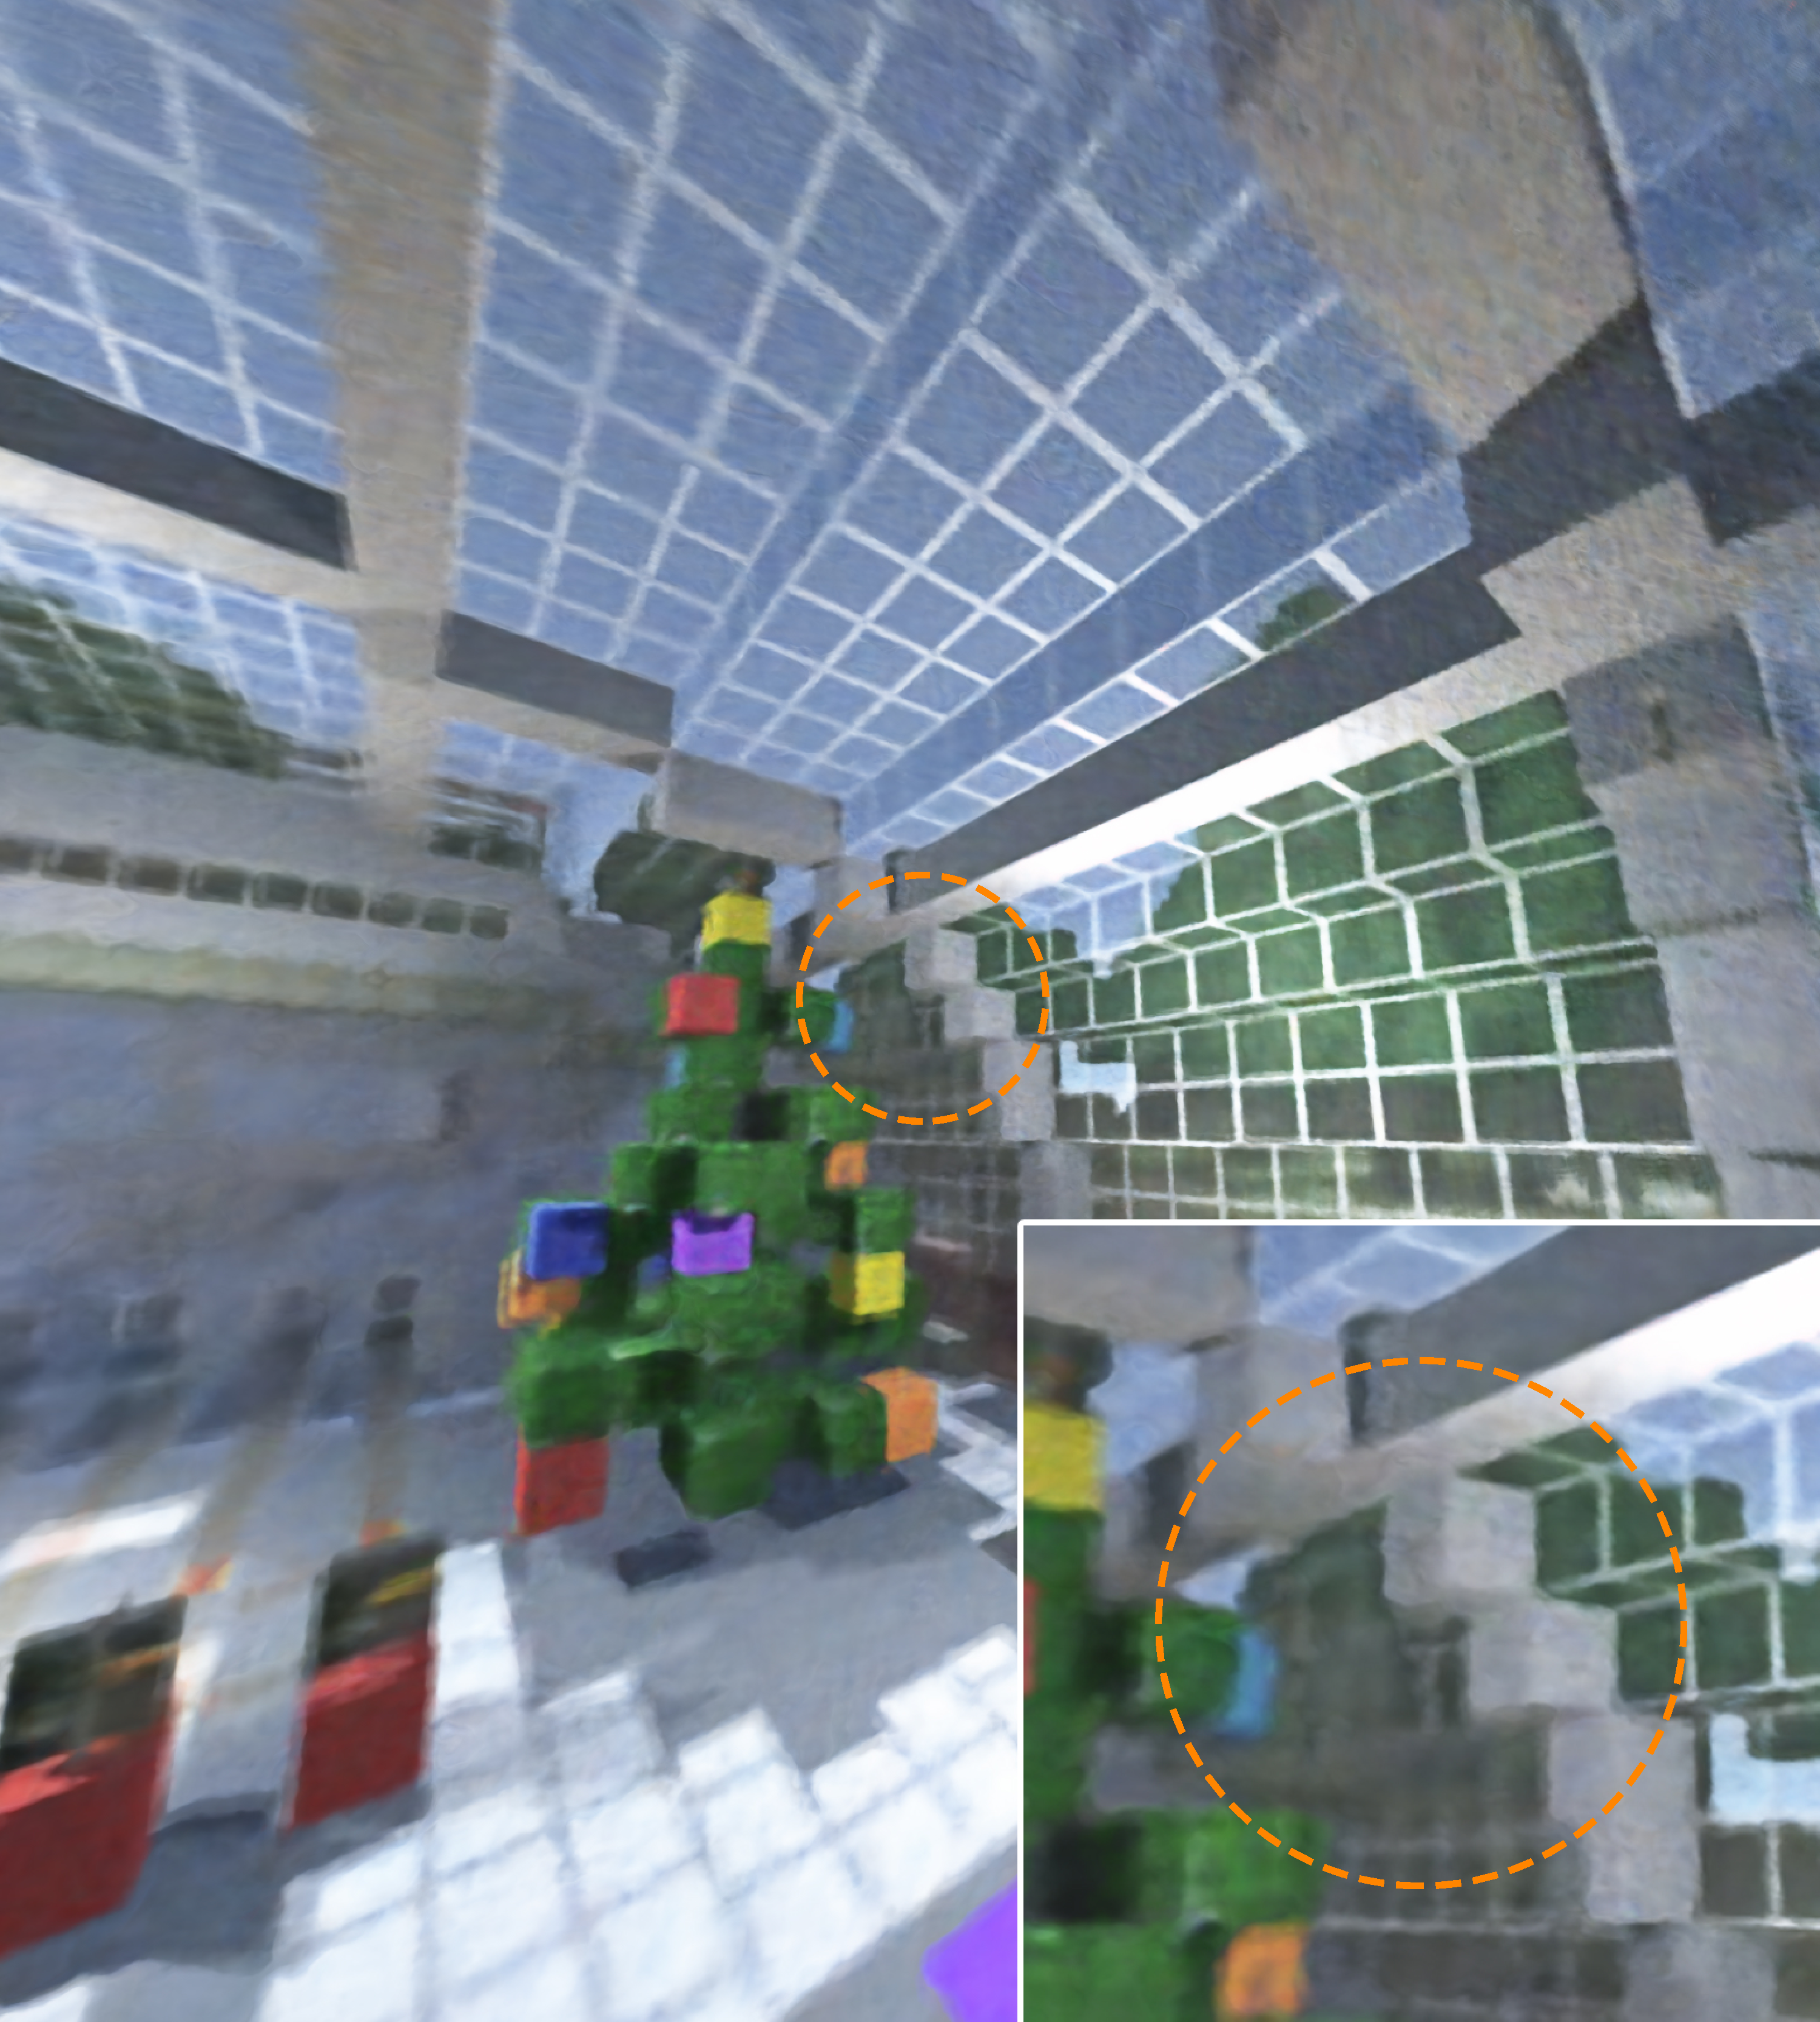
\includegraphics[width=0.96\linewidth]{TOG/figs/mc_nerf3_inset.pdf}}
        
        \subfloat[bedroom scene (\textbf{NeRF})]{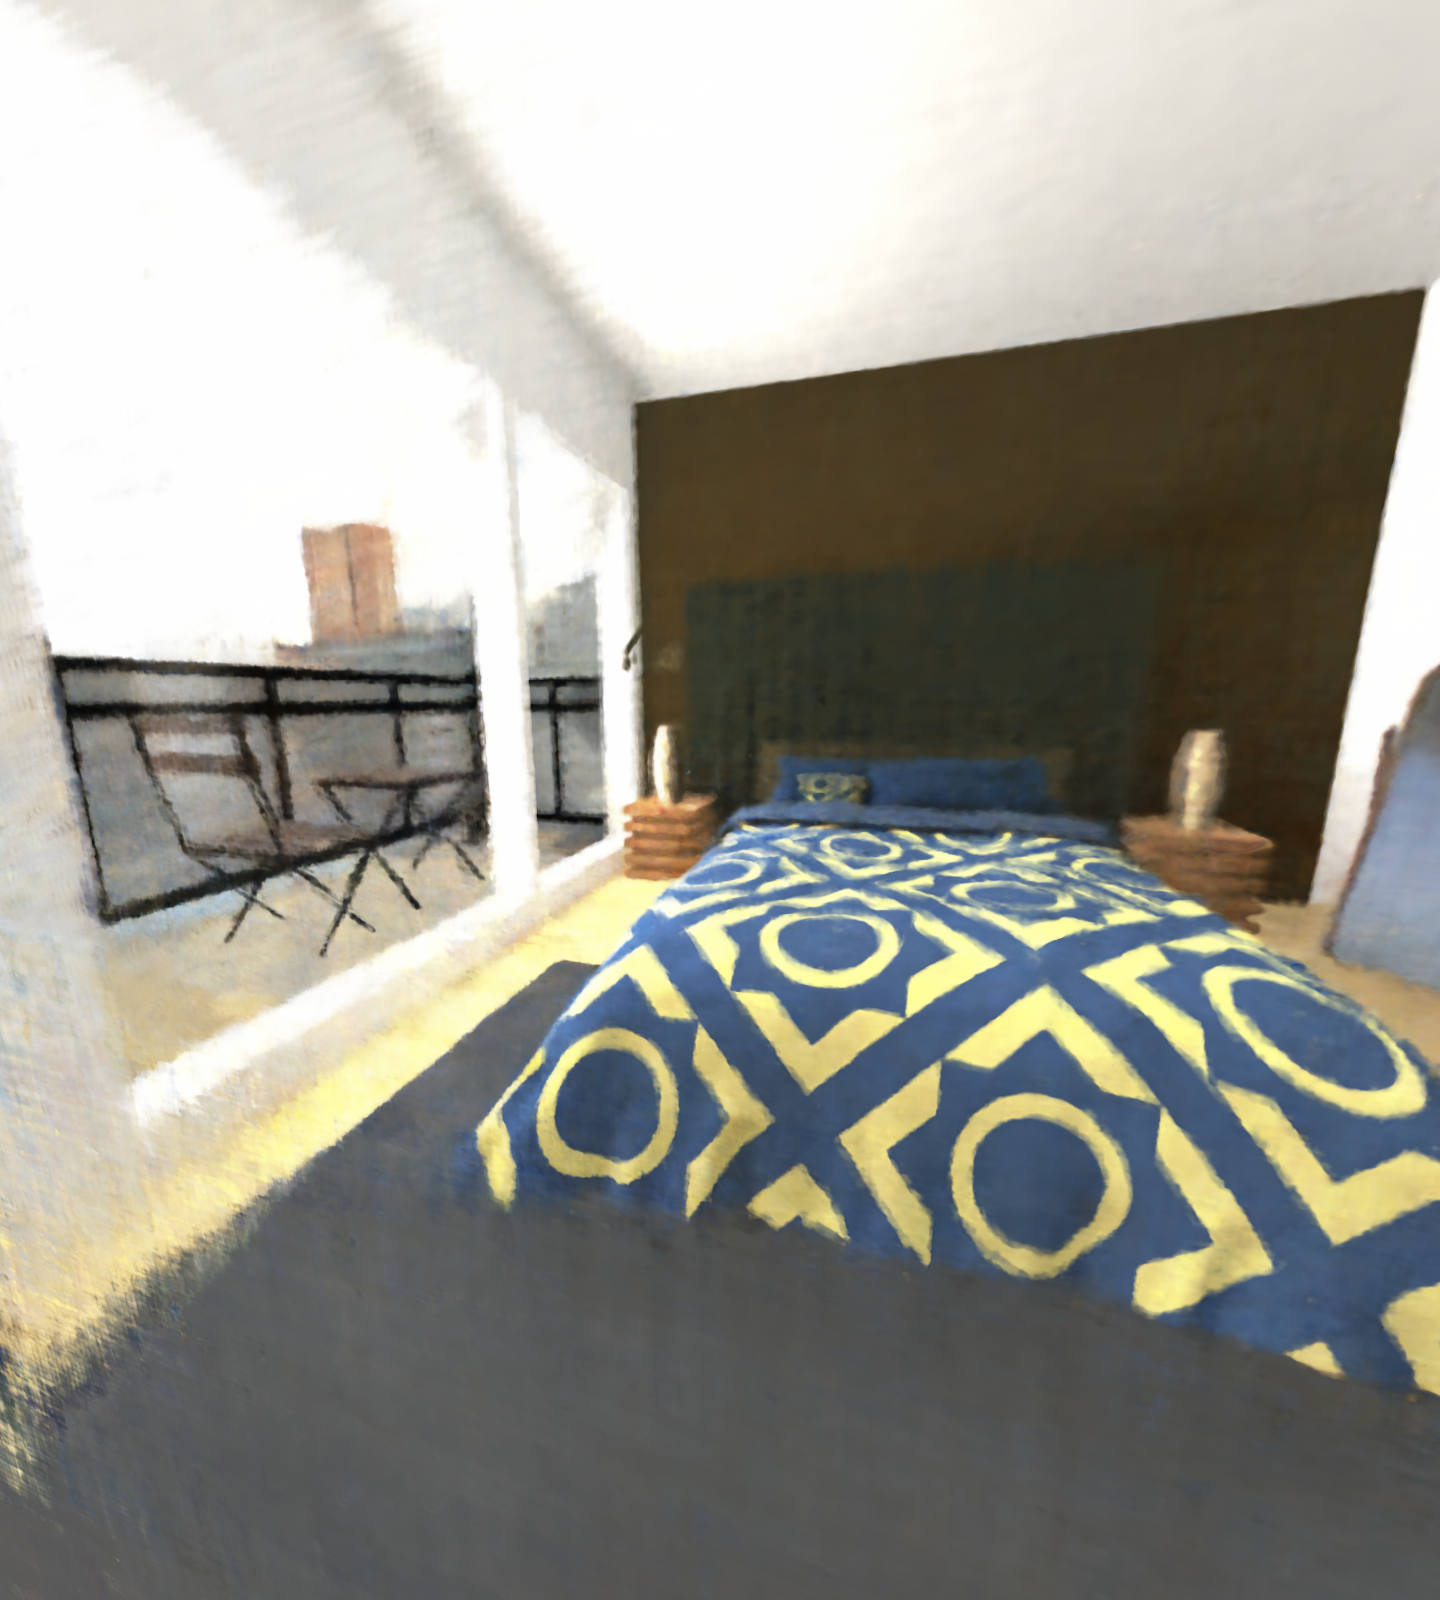
\includegraphics[width=0.96\linewidth]{TOG/figs/bed_nerf0.png}}      
    \end{minipage}    
    
    \caption{Comparing our synthesis method (2nd column) with full resolution (1st column) rendering and NeRF (3rd column).}
    % {\zh{add inset for 2nd and 3rd col}}
    \label{fig:results:comparison}
\end{figure*}

\begin{figure*}[htb]
    \centering
    \begin{minipage}{0.32\linewidth} %full res
        
        \subfloat[gallery scene (\textbf{GT})]{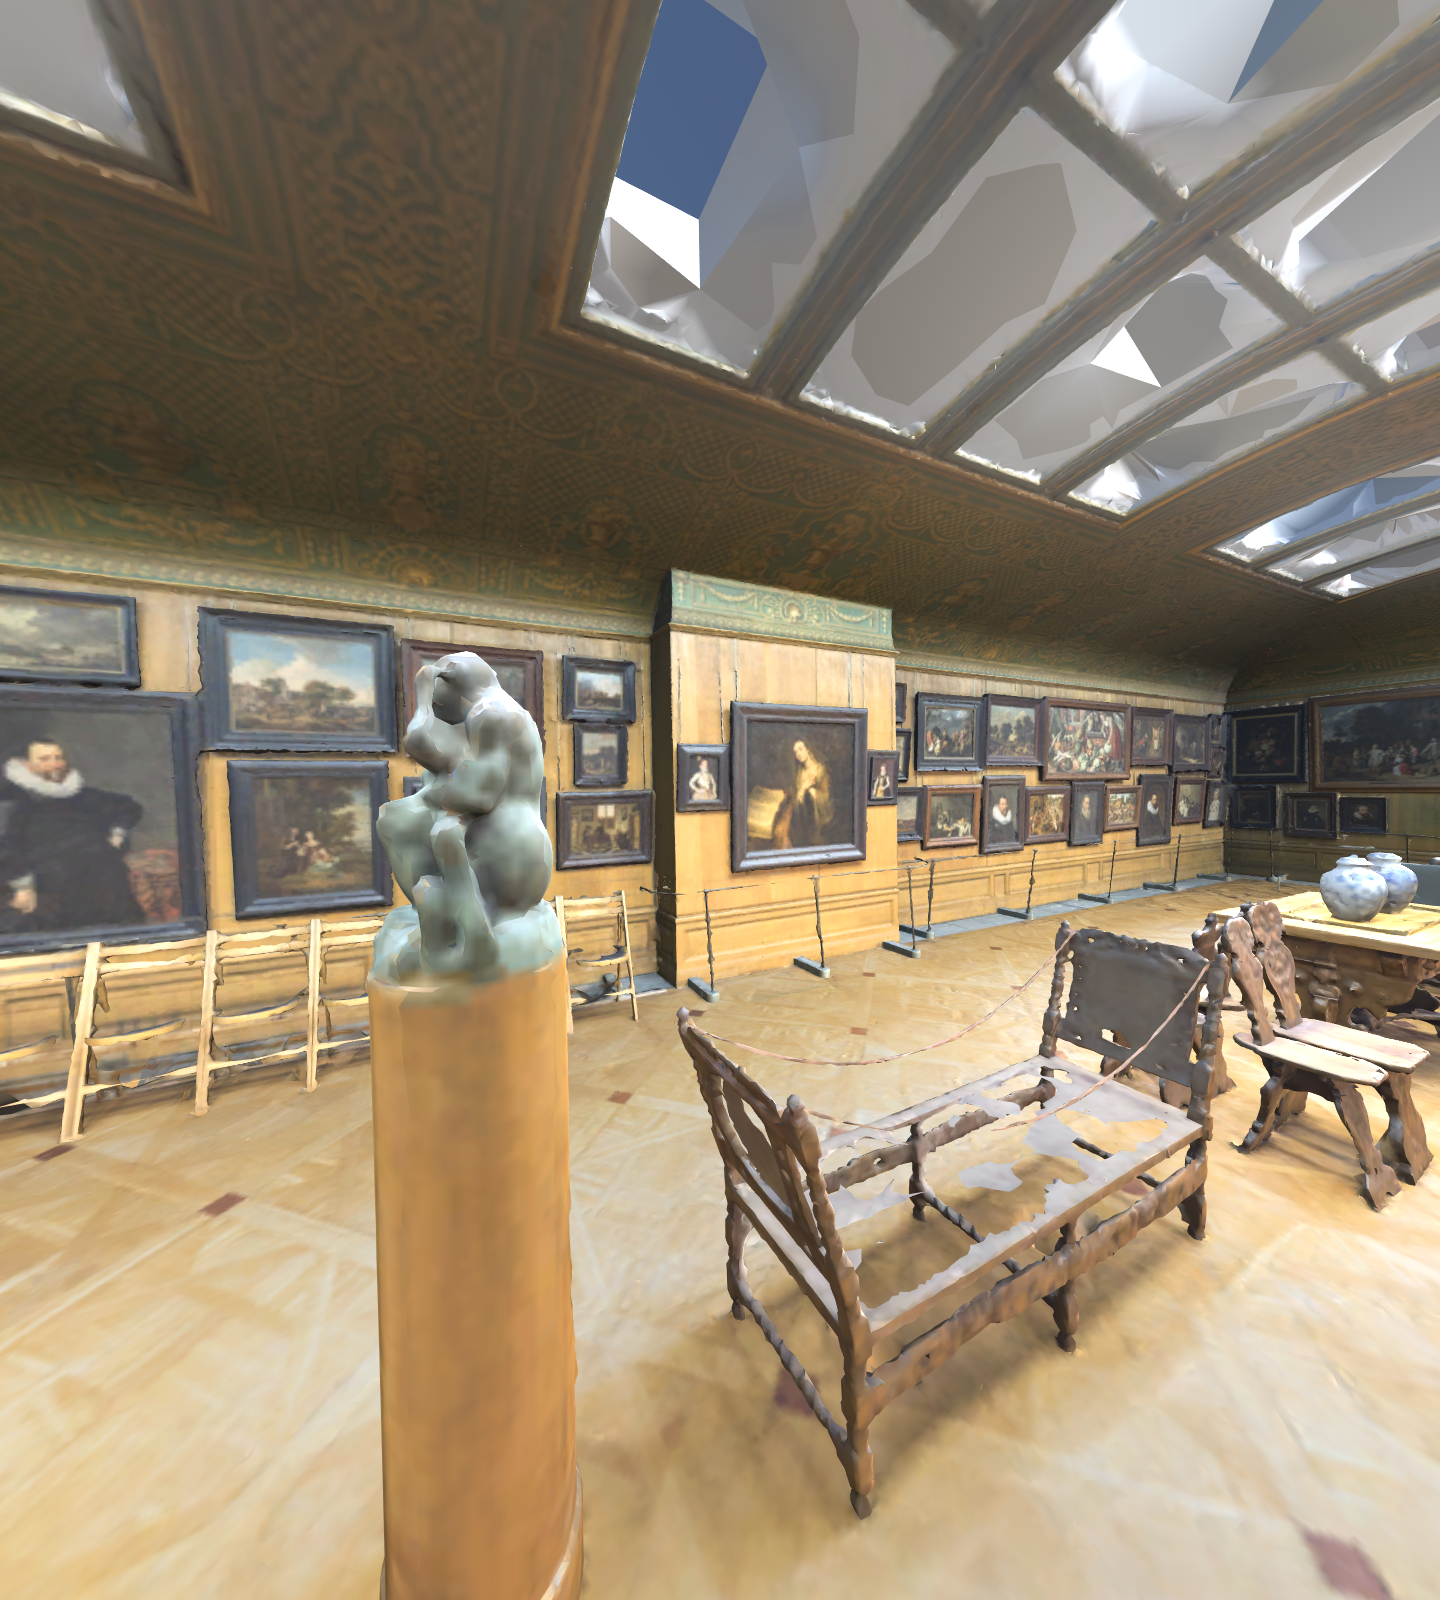
\includegraphics[width=0.96\linewidth]{TOG/figs/gallery_GT_view_0001.png}}
    \end{minipage}
    \begin{minipage}{0.32\linewidth} %ours
        
        \subfloat[gallery scene (\textbf{OUR})]{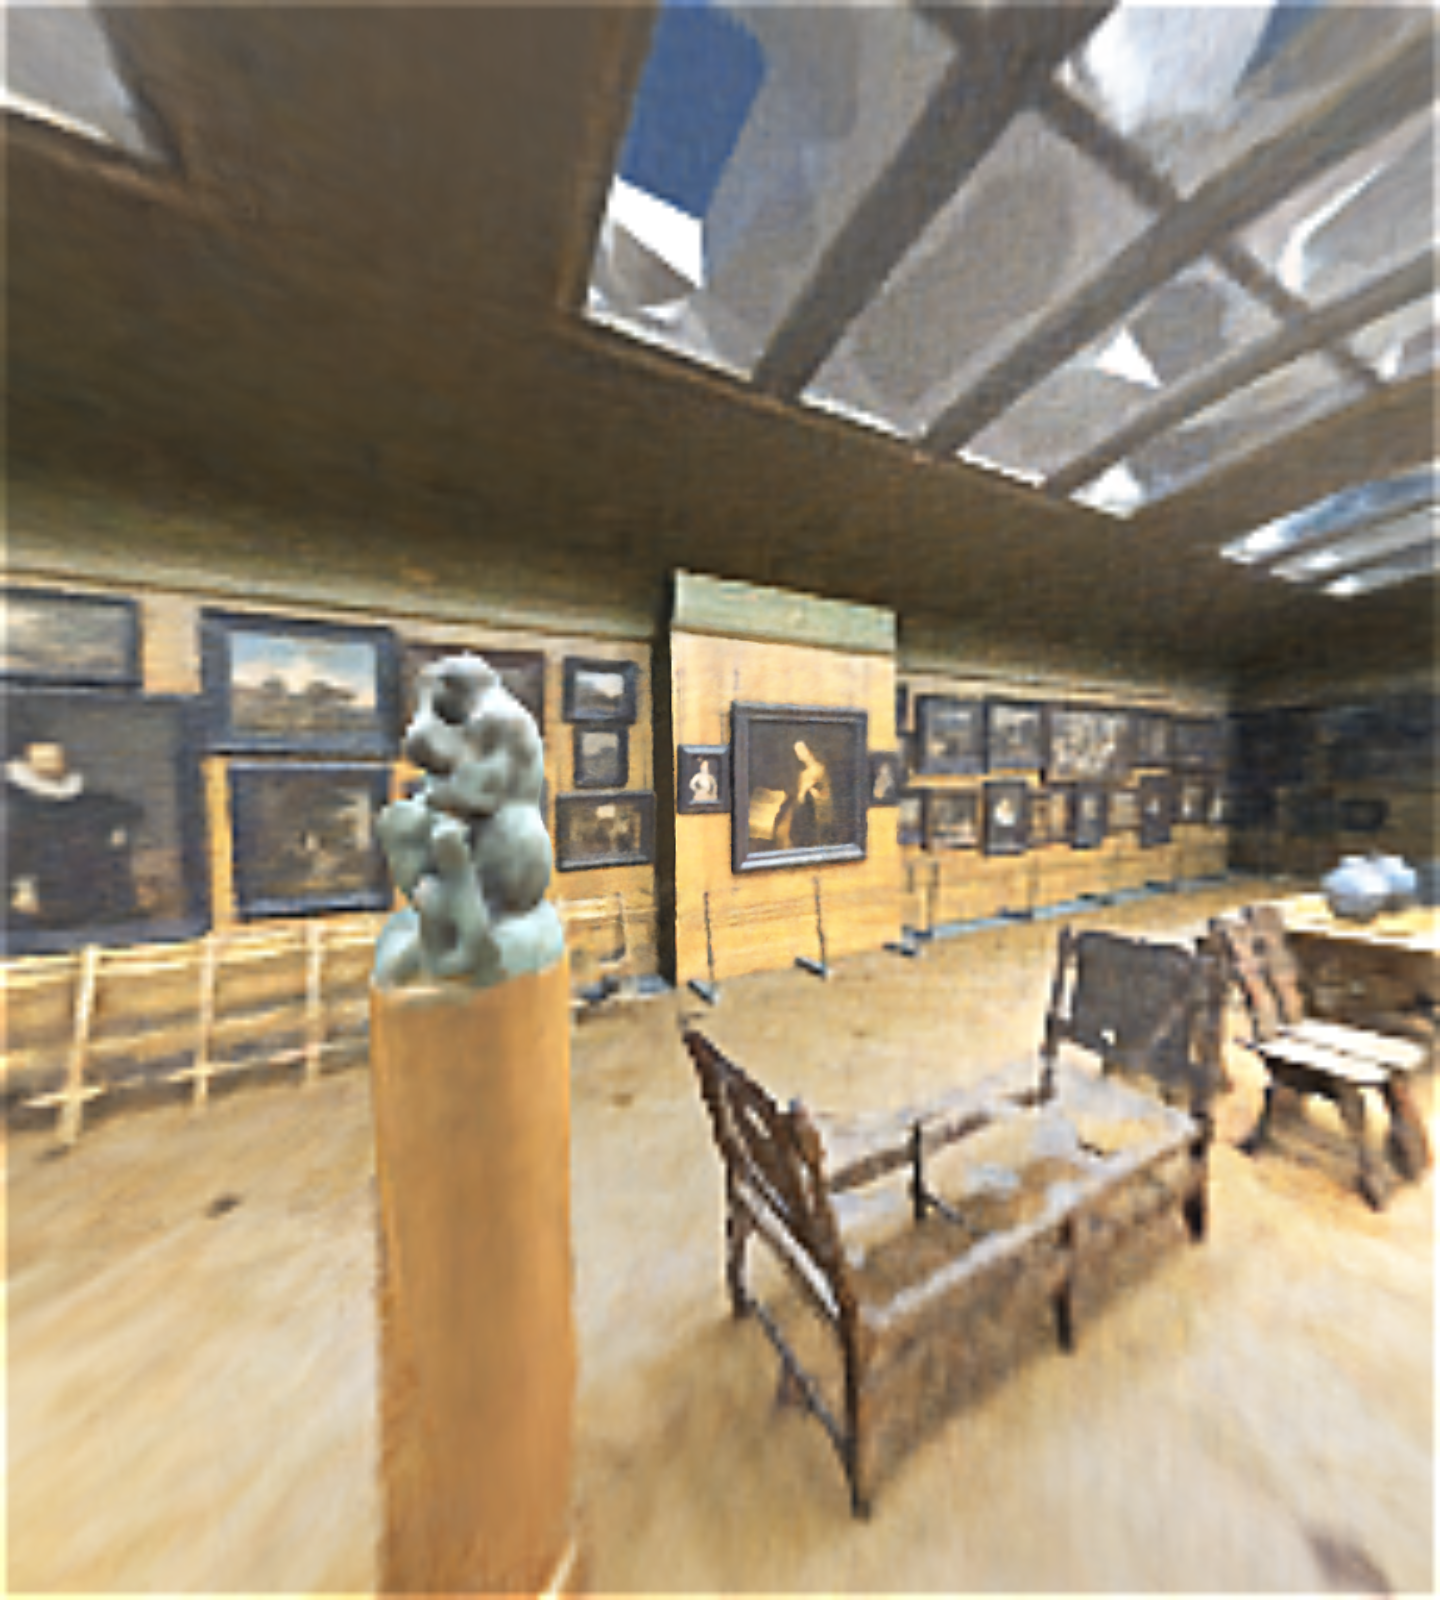
\includegraphics[width=0.96\linewidth]{TOG/figs/gallery_our_001.png}}                
    \end{minipage}
    \begin{minipage}{0.32\linewidth} % NERF
        
        \subfloat[gallery scene (\textbf{NeRF})]{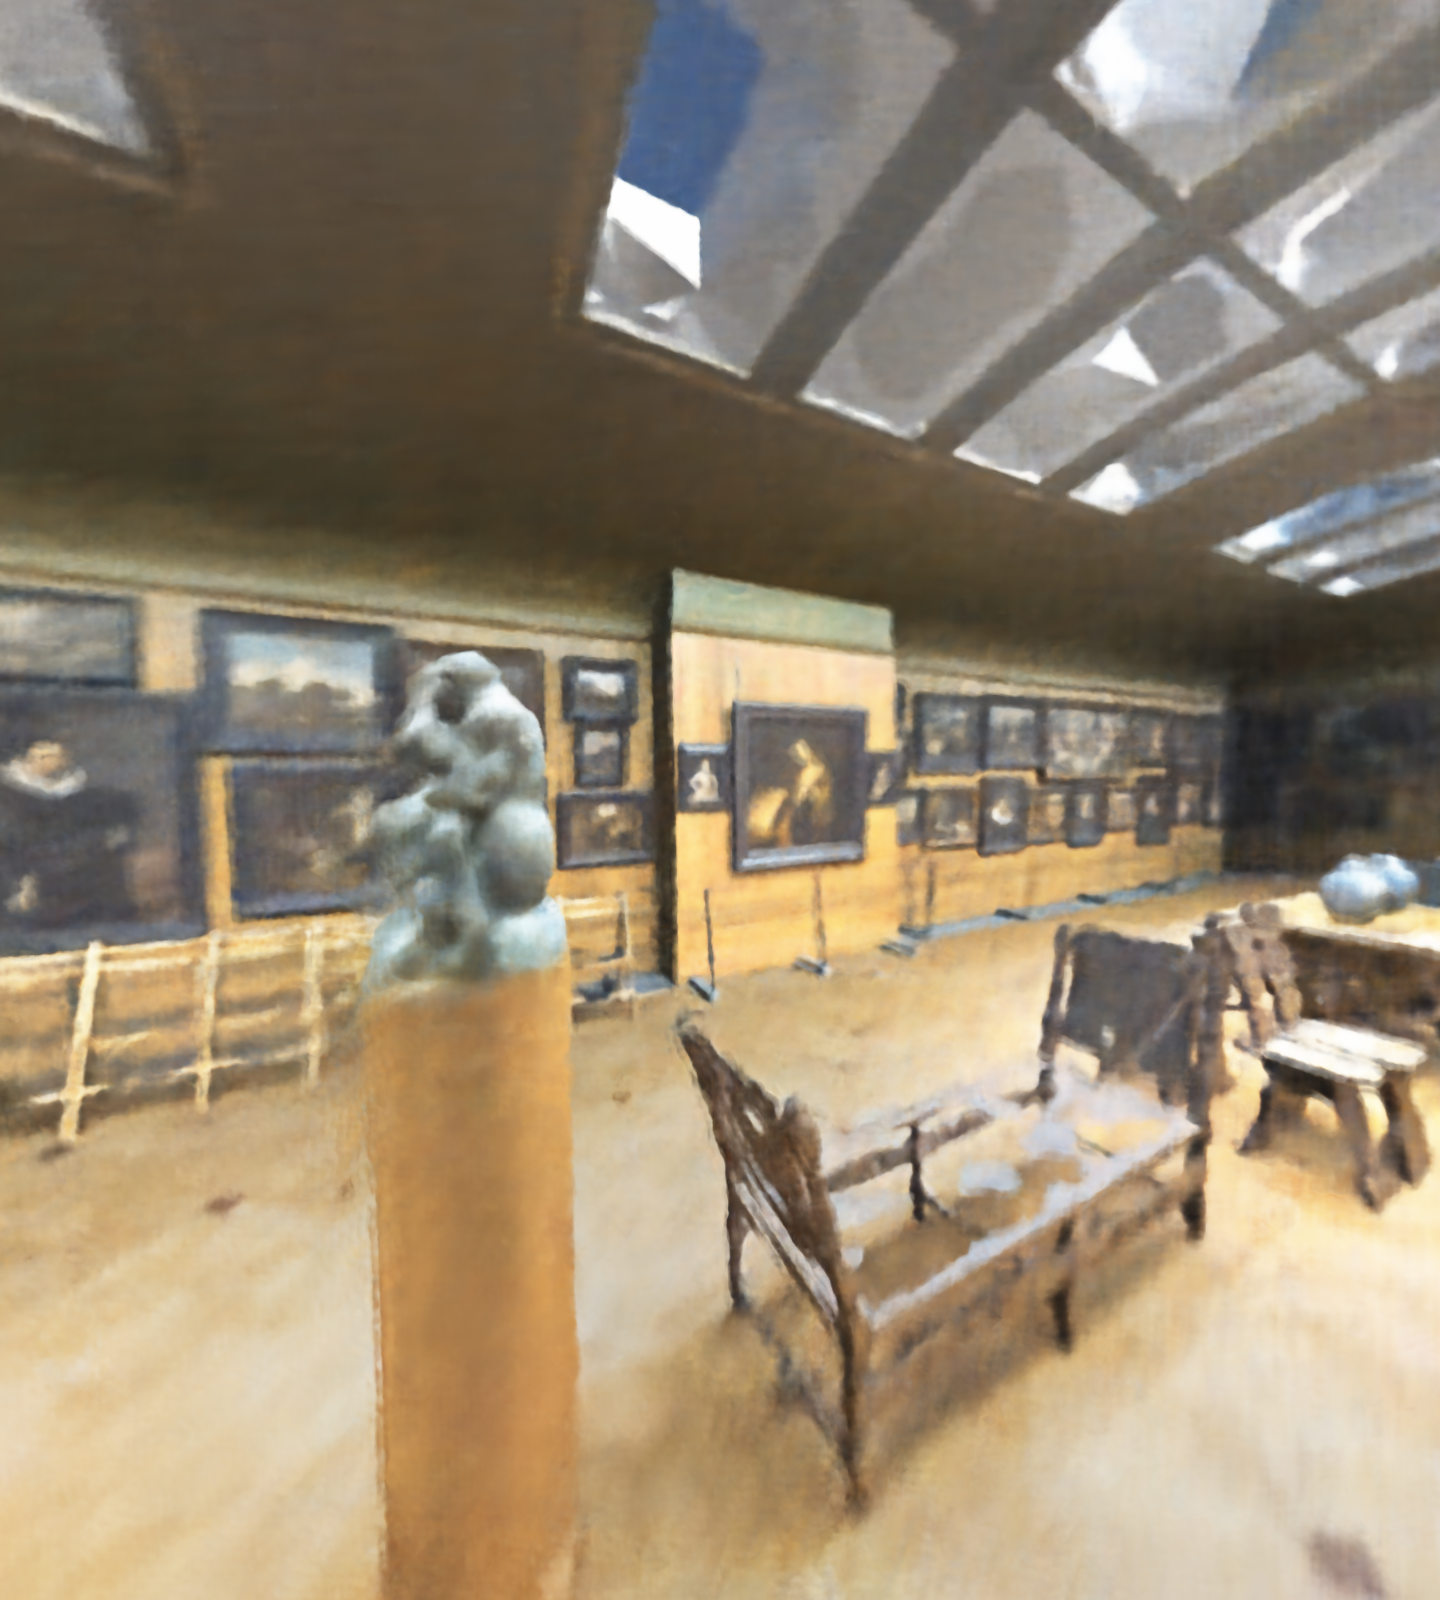
\includegraphics[width=0.96\linewidth]{TOG/figs/gallery_NeRF_001.png}}        
    \end{minipage}    
    
    \caption{Comparing our synthesis method (2nd column) with full resolution (1st column) rendering and NeRF (3rd column). (Cont.).}
    % {\zh{add inset for 2nd and 3rd col}}
    \label{fig:results:comparison2}
\end{figure*}
With a variety of scenes as shown in \Cref{fig:results:comparison}, we first conduct subjective studies (\Cref{sec:study:user}) and objective measurements (\Cref{sec:study:quality}) to evaluate the perceptual quality.
Further, we analyze the intra-system workings and compare inter-system performance in \Cref{sec:study:intra}.

\subsection{User Study}
\label{sec:study:user}
% \zh{(Jan 10) all the Qs are answered offline, will update the section soon.}
% In this section, we report two perceptual experiments to investigate 1) how users perceive our solution and the ground truth and 2) how our solutions behaves compared to other alternatives.
We first conducted a psychophysical experiment to investigate how users perceive our solution ({\bf OURS}) compared with existing neural view synthesis methods (\cite{mildenhall2020nerf}, {\bf NeRF}) and foveated rendering with the full mesh data (\cite{perry2002gaze}, {\bf F-GT}).

% \zh{usually we report the study design here too, like within-subject user study and analyze method, like ANOVA. But I am not sure what we should use here.}
% \zh{(Jan 12), if we include NeRF, I'd say we keep one of the down-sample conditions}

\paragraph{Stimuli}
For precise comparison and accommodating the low frame rate of alternative solutions (as to be compared in \Cref{sec:study:intra}), each group of stimuli were static images rendered via {\bf F-GT} or synthesized via  {\bf OURS}/{\bf NeRF} with the same views, as shown in \Cref{fig:results:comparison}.
They were generated with the same and randomly defined gaze fixation across conditions.
The resolution of the image per eye was $1440 \times 1600$. 
During the study, the target gaze position was indicated as a green cross on the stimuli images.
% The resolution of the images per eye was $1440 \times 1600$. 
We used the {\it gas} and {\it minecraft} scenes for the diverse indoor/outdoor environment.
Each condition from an individual scene consists of \nothing{$1$ view and} $3$ different gaze positions.

The foveal kernel size in {\bf F-GT} was designed to match our display size and eye-display distances.
For generating {\bf NeRF} condition, we retrained the model from \cite{mildenhall2020nerf} on our dataset with $N_{sample}=16$, $N_{layers}=4$, $N_{channel}=128$. The bottom right of each scene figure \Cref{fig:results:comparison} shows the resulting images. 
%We predict the image from the camera transformation, fine-tune the foveated layer, and render the image by alpha blending the three layers.

%\zh{We probably don't need to attach foveated GT here}
% The second column is a uniformly down-sample image at size \warning{??? x ???}. Assuming our network bandwidth is \warning{???}, to stream the images from the cloud in real time, the largest size of the image per eye is up to \warning{??? = ??? / 50 fps / 2 eyes}. So we down sample the entire image with ratio \warning{???}.
%The second column enables foveated rendering. We applied \warning{foveated algorithms} described in \cite{perry2002gaze} and \cite{jiang2015salicon}. 
% and The foveated area is preserved as the original resolution while the rest of the image is down sampled. same alpha blending method that we used in our solution (see \autoref{sec:method:blending}). Similarly, we calculate the size of the foveated image based on the bandwidth. Hence the down-sample ratio of peripheral area is \warning{???}. 
%The third column is generated by NeRF implementation. We retrained a new model on our dataset with parameters $N_{sample}=16$, $N_{layers}=4$, $N_{channel}=128$. The last column is our result. We predict the image from the camera transformation, fine-tune the foveated layer, and render the image by alpha blending the three layers.

\paragraph{Setup}
Each participant wore an eye-tracked HTC Vive Pro Eye headset and remained seated to example the stimuli during the experiment.
Ten users participated in and completed the study (3 females, $M=23.7$, $SD=1.49$). 
% One participant (age=23, female) did not complete the experiment due to constant gaze drifting (please refer to the task description below).
None of the subjects were aware of the research, the experimental hypothesis, nor the number of methods. All participants had a normal or corrected-to-normal vision.

\paragraph{Task}
The task was a \textit{two-alternative-forced-choice} (2AFC). Each trial consists of a pair of stimuli generated from two of the three methods ({\bf OURS} / {\bf NeRF} / {\bf F-GT}) with a sampled view and gaze position. Each stimulus appeared for $300$ms on display. A forced $1.5$sec break (black screen) was introduced between conditions to clear the vision. During the study, the participants were instructed to fix their gazes on the green cross. To prevent the fixation from shifting away and ensure accuracy, we tracked the users' gaze throughout the experiment. Whenever the gaze is more than $5$deg away from the target, a trial was dropped immediately with a black screen informing the participant.
After each trial, the participants were instructed to select which of the two stimuli appeared with higher visual quality using a keyboard.
Before each experiment, a warm-up session with 6 trials was provided to familiarize the participants with the study procedure. The orders of conditions among trials were randomized with counterbalancing. The entire experiment of each user consists of $36$ trials, $12$ trial per pair of conditions.
%To start with, each participant was informed that they were required to choose an alternative with higher quality after watching each pair of stimuli. We calibrated the device and performed a warm-up trial to help participants understand our system. Each participant were provided with 1 warm-up trial and 6 official trials (2 scenes x 1 view x 3 gaze positions) where each trial consisted all the combinations of the pairs of every two stimuli. We randomize the order of the pairs for counterbalancing. We showed a yellow cross on the screen. After participants move their gaze positions to the area close to the cross, the yellow cross turns green. The first stimulus will be rendered as well as the cross after participants fixate the cross for 1 second. Each stimulus is displayed for 300 milliseconds. The second one will be rendered after 1.5-second dark screen. If the participants does not fixate at the cross when stimuli are displayed, the current pair will be discarded and displayed to the participants later in the same trial. After each pair, participants reported their opinions on which image has higher quality.
To minimize the effect of accumulated fatigue, we enforced breaks at least a 2-second between trials and 60-second after each scene. Meanwhile, the participants were able to take as much time as needed. 

\paragraph{Results}
\begin{figure}[ht]
    \centering
    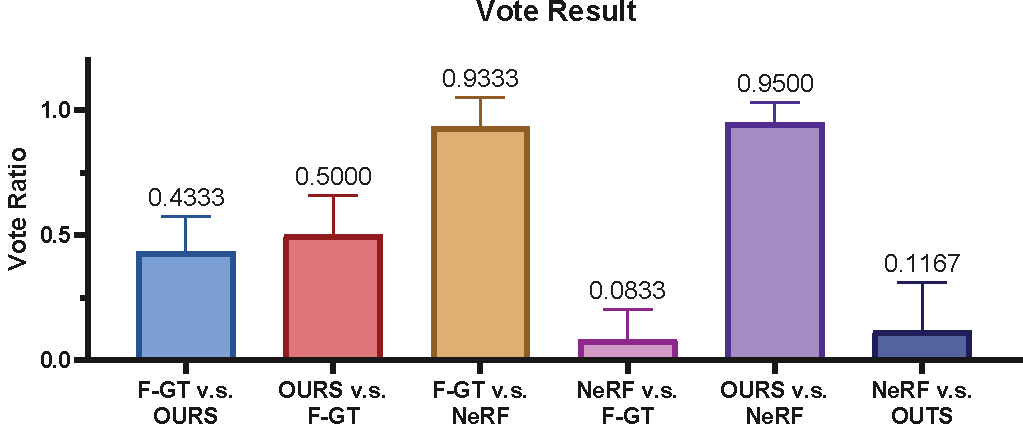
\includegraphics[width=0.96\linewidth]{TOG/figs/vote-average-mono.pdf}
    \Caption{The users' preference votes from our evaluation experiment (\protect\Cref{sec:study:user}).}
    {%
    X-axis shows all pairs of conditions (rendering/synthesis methods and their orders in the 2AFC); Y-axis shows the ratio of voting for the first one in each pair.
    }
    \label{fig:results:2afc}
\end{figure}
\Cref{fig:results:2afc} plots the results considering both methods and their orders in the 2AFC experiments. Among all three conditions, we observed close-to-random-guess among trails that compares {\bf F-GT} and {\bf OURS} ($53.3\%$ voted for {\bf OURS}, $SD=14.9\%$). Meanwhile, a significantly higher ratio of voting {\bf F-GT} over {\bf NeRF} was observed ($92.5\%$, voted for {\bf F-GT}, $SD=11.4\%$, binomial test showed $p<0.005^{***}$). The preference applies to {\bf OURS} vs. {\bf NeRF} as well ($91.7\%$ voted for {\bf OURS}, $SD=14.8\%$, binomial test showed $p<0.005^{***}$).
% \qisun{(Jan 23, 2021) @Zhenyi: consider adding stdev to the average numbers above? This shall be reflected in \Cref{fig:results:2afc} as well. Also, double check the numbers between here and the plot as they are not matching now.}

% our/gt 78/156 0.5318897993488445
% our/nerf 152/156 2.6681140960754964e-40
% nerf/gt 2/156 1.3407579916082842e-43
% our/gt 64/120 0.26149549194499716
% our/nerf 110/120 9.586645257178695e-23
% nerf/gt 9/120 8.546460059714397e-24

% apply binomial test https://docs.scipy.org/doc/scipy/reference/generated/scipy.stats.binom_test.html
% or apply ANOVA, there is a value of votes for each condition and we want to know if there exists significant effects on different condition.
\paragraph{Discussion}
The close-to-random-guess indicated the statistically similar perceptual quality between {\bf OURS} and foveated ground truth ({\bf F-GT}). 
Given the perceptual identicality between foveated and full-resolution rendering, the subjective study reveals that {\bf OURS} can achieve similar quality as a rendering with locally fully stored high-quality 3D data.

Meanwhile, both of the two conditions showed significant quality preference than {\bf NeRF}. That is, with immersive, high FoV, and first-person viewing constraints, {\bf OURS} synthesizes gaze-contingent retinal image with superior perceptual quality than alternative synthesis solutions. The latter typically aims to reconstruct the full image over the entire field-of-view. \nothing{the current volume-based scene representation may not fully reproduce the perceptually identical retinal images.}
To further validate the perceptual quality at individual eccentricities across the whole visual field, we analyze with objective metrics in the following section.

\subsection{Visual Quality}
\label{sec:study:quality}
\begin{figure*}
    \centering
    \subfloat[gas]{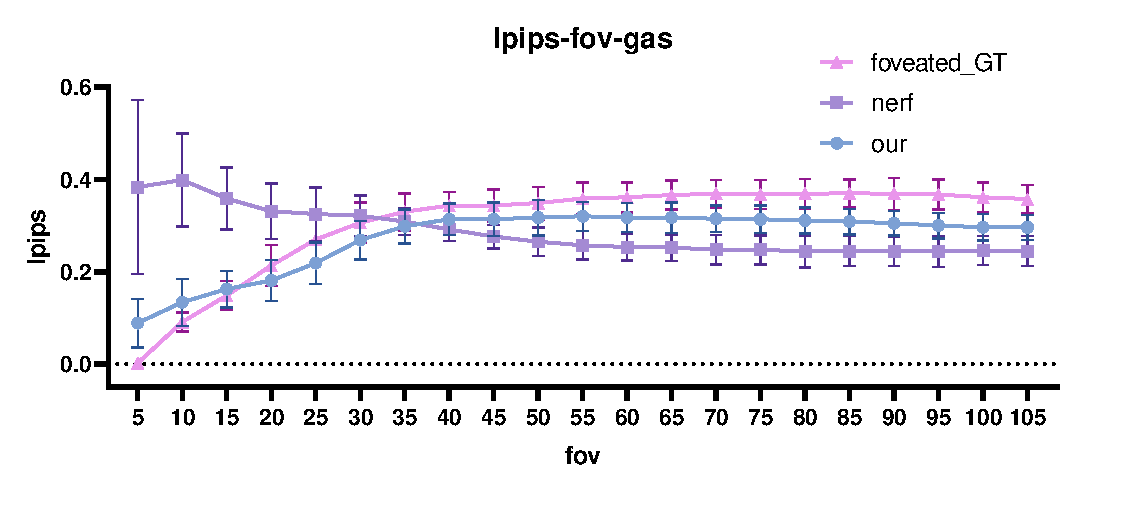
\includegraphics[width=0.48\linewidth]{TOG/figs/lpips-fov-gas-group.pdf}}\label{lpips:gas}
    \subfloat[minecraft]{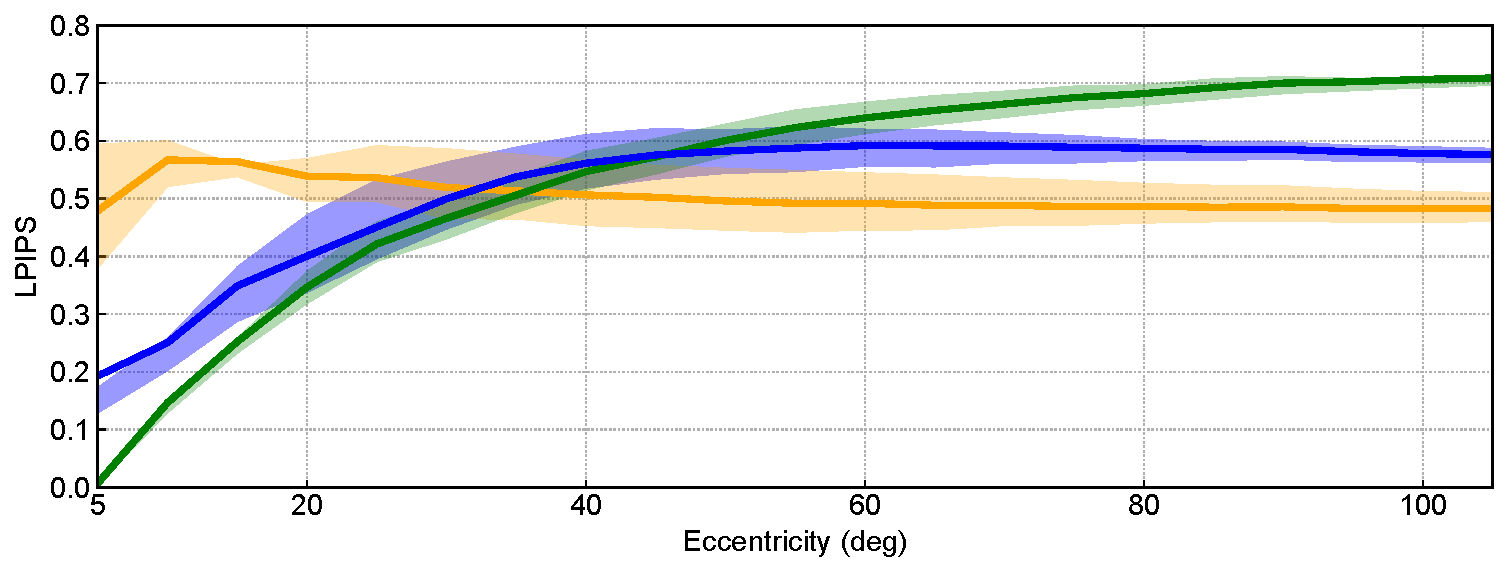
\includegraphics[width=0.48\linewidth]{TOG/figs/lpips_scenemc.pdf}}
    
    \subfloat[studyroom]{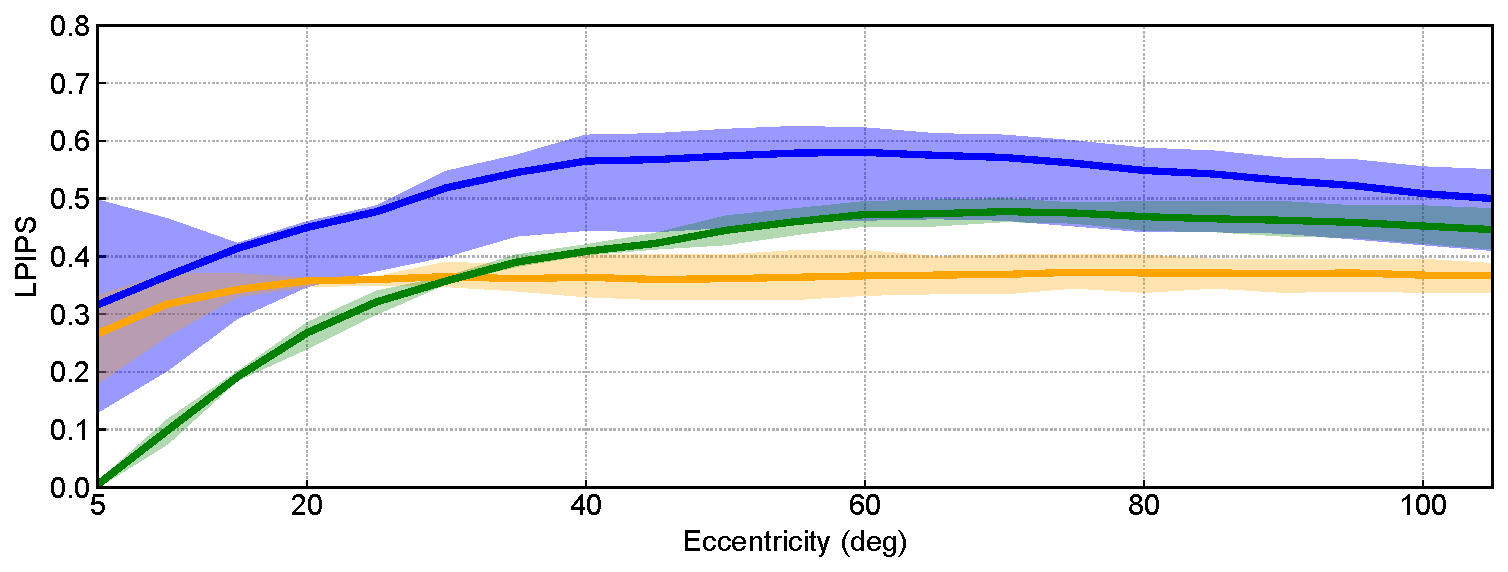
\includegraphics[width=0.48\linewidth]{TOG/figs/lpips_scenestudyroom.pdf}}
    \subfloat[bedroom]{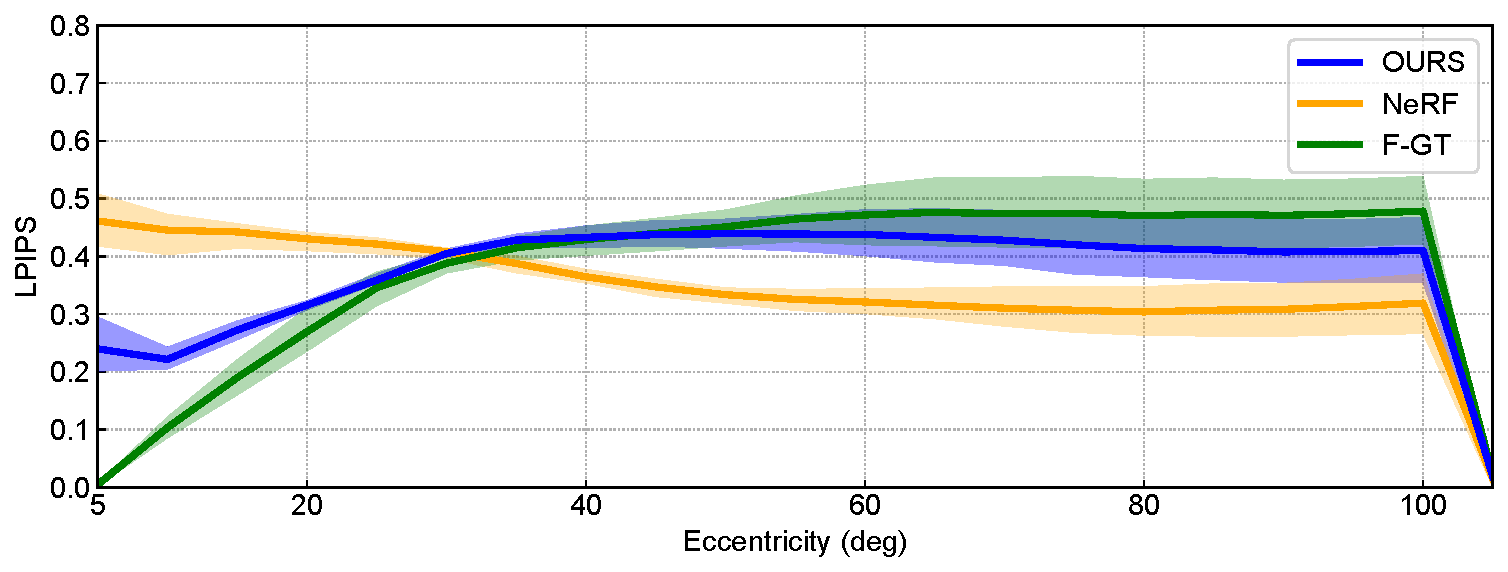
\includegraphics[width=0.48\linewidth]{TOG/figs/lpips_scenebedroom.pdf}}
    \caption{LPIPS analysis of all scenes as well as comparison of our method, NeRF, and foveated GT on each eccentricity. $^*$: $p<.05$, $^{**}$: $p<.01$.}
    {We found a significant difference in \warning{ecc range} between \warning{stimulus} and \warning{stimulus};}
    \label{fig:lpips}
\end{figure*}
Complementary to the subjective measurement (\Cref{sec:study:user}), we evaluate the perceived quality in an objective fashion. Specifically, under all four different scenes (indoor/outdoor, artificial/realistic), we compare {\bf OURS}, {\bf F-GT} and {\bf NeRF} at individual eccentricity ranges (up to $110$ deg, the capability of the VR HMD) via partial images. 
For each eccentricity range, we compare the deep perceptual similarity (LPIPS) \cite{zhang2018unreasonable} across all scenes. LPIPS uses deep neural networks to estimate perceptual similarities between the image provided and a reference image. Smaller values indicate higher perceptual similarity.
For each scene, we sample $20$ views with gazes at the middle of the display, resulting in $20$ data per eccentricity value, $420$ data per scene. We used one-way repeated measures ANOVAs to compare effects across three stimuli on each eccentricity range and together. Paired t-tests with Holm correction were used for all pairwise comparisons between stimuli. All tests for significance were made at the $\alpha=0.05$ level. 
% The error bars in the graphs show the 95\% confidence intervals of the means.

\paragraph{Results} 
% \warning{need to update}
\Cref{fig:lpips} plots LPIPS values across all scenes and eccentricity ranges ($5$ deg step size). 
From foveal to near eccentricity (<=$40$ deg), we observed significant effects of the stimuli on LPIPS with a ``large'' effect size ($\eta^2 = 0.26$). That is, \textbf{OURS} shows significantly lower LPIPS than \textbf{NeRF} ($p<.001^{***}$), although higher than \textbf{F-GT} ($p<.001^{***}$).
For example, the main effects of stimuli ($F(2,38)=210.76, p<.001^{***}$) was significant on eccentricity $=[0,25]$ deg in scene \textit{gallery} (\Cref{fig:lpips:gallery}). \textbf{OURS} was significantly lower than \textbf{NeRF} ($t(19)=-19.54, p<.001^{***}$) and \textbf{F-GT} ($t(19)=-4.32, p<.001^{***}$) both with a ``large'' effect size (Cohen's d $>0.8$). The example observation generally applies to all 4 scenes being validated. 

From mid- to far- periphery (>$40$ deg), we observed significant effects of the stimuli on LPIPS with a ``large'' effect size ($\omega^2 = 0.16$). \textbf{OURS} shows significantly higher LPIPS than \textbf{NeRF}. Whereas, comparing with \textbf{F-GT}, we observed significant lower scores ($p<.001^{***}$).
For instance, the main effects of stimuli was significant on eccentricity $=60$ deg in scene \textit{bedroom} ($F(2,38)=411.93, p<.001^{***}$, \Cref{fig:lpips:bedroom}). \textbf{OURS} was significantly lower than \textbf{F-GT} ($t(19)=-3.78, p<.001^{***}$), and higher than \textbf{NeRF} ($t(19)=22.75, p<.001^{***}$) both with a ``large'' effect size (Cohen's d $>0.8$). The example observation generally applies to all 4 scenes being validated. 

\paragraph{Discussion}
In the fovea and near-periphery, the observation revealed our method's significantly higher perceptual quality than alternative neural representation solutions. This is evidenced by the significantly stronger perceptual similarity to \textbf{F-GT} by comparing between \textbf{OURS} and \textbf{NeRF}. The subjective study (\Cref{sec:study:user}) evidenced the marginally lower similarity than \textbf{F-GT} as statistically unnoticeable among users.

In the far-periphery, \textbf{OURS} showed increased LIPIPS than \textbf{F-GT} beyond $40$ deg.
The latter has been shown to display identical perceptual similarity than full resolution rendering in VR \cite{Patney:2016:TFR}.
Thus, the findings show that \textbf{OURS} doesn't compromise the peripheral vision's quality with its significantly enhanced synthesis acuity in fovea. 

Note that the discoveries also agree with the observations from \Cref{sec:study:user}. That is, in addition to the significantly faster performance  ($99.7\%$ time reduction per frame as in \Cref{sec:study:intra}\nothing{\qisun{Check if I noted it right.}}), our method showed superior perceptual quality than \textbf{NeRF} under first-person, high resolution, and immersive viewing of 3D scenes. Meanwhile, our synthesized views are perceptually identical to the traditionally rendered images with a complete 3D mesh. It yet achieves significant data storage-saving with only about $0.5$mb (up to $99.5\%$ in our experiment).

\subsection{Performance}
\label{sec:study:intra}
% apply objective metric to |cref{fig:optimization}, aka different sample numbers
Virtual and augmented reality demands high frame rates along with high quality to ensure immersive and comfortable experience. Our neural synthesis method introduces both spatial and angular (stereo) visual perception for real-time performance (\Cref{sec:method:representation}). 
Further, our precision-latency joint optimization for the representation and network also balances quality and performance.
Here, we evaluate the performance of each component in our system and compare with existing neural synthesis solutions.

For high resolution ($1440\times1600$), high field-of-view ($110$deg) stereo images required by VR display, our system completes all computation (including gaze-contingent neural-inference and elemental images composition) in $31.8$ms per frame without stereo foveation, \dncR{as shown in \Cref{tbl:ablation} \st{shows a time consumption breakdown of our method, together with {\bf NeRF}}}. Compared with {\bf NeRF} \dncR{(the bottom row of \Cref{tbl:ablation})}, our spatial foveation \dncR{\st{for adaptive resolution}} significantly improves the system performance from offline computation (in seconds) to interactive speed (\dncR{about 30 frames per second\st{$31.8$ ms per frame}}).

Tailored for VR displays, our \dncR{stereo foveation\st{adaptive stereo synthesis}} further reduces the computation time \dncR{and achieves high performance of more than 50 frames per second \st{by more than $10$ms/frame}}, contributing to a temporally continuous viewing experience without loss of perceived resolution and quality.

%Specifically, the significant performance gain benefits from the spatial and stereo foveation that do not compromise the visual quality.
\begin{table}[!htb]
    \centering
    \begin{tabular}{ l|r } 
        \toprule
         foveal infer (per eye)  & 3.8 \\
         \midrule
         periphery infer (per eye) & 11.9 \\
          \midrule
         blending \& contrast enhancement & 0.2 \\
          \midrule\midrule
         {\bf OUR} method without stereo foveation & 31.8\\
         {\bf OUR} full method & {\bf 19.7}\\
         \midrule
         {\bf NeRF} \cite{mildenhall2020nerf} & $9\times10^3$ \\
         \bottomrule
    \end{tabular}
    \Caption{Time consumption breakdown and comparison.}
    {%
    The numbers show the time consumption of each component and the overall system per frame. All units are in millisecond.
    \nothing{\qisun{(Jan 25) I have update the time consumption of {\bf NeRF}. See if that is correct.}}
    }
    \label{tbl:ablation}
\end{table}

% \begin{table*}[!htb]
%     \centering
%     \begin{tabular}{ |c|c|c|c|c|c|c| } 
%         \hline
%          & foveal infer & periphery infer & blending & contrast & system without mono-periphery & system with mono-periphery \\
%         \hline
%         without sub-net & \warning{3.2\times2} & \warning{10} & \multirow{2}{3em}{\warning{2}} & \multirow{2}{3em}{\warning{2}} & 30.4 & 20.4 \\ 
%         with sub-net& 3.5 & 12 & & & 35 & 23 \\ 
%         \hline
%     \end{tabular}
%     \caption{Performance.}
%     \label{tbl:ablation}
% \end{table*}

% \paragraph{sub-net}
% As described in \cref{sec:method:optimization} and \Cref{sec:impl}, we find the optimal parameters for our network and further split the network into two sub-nets based on the distance. Without sub-net, it takes \warning{3.2}ms to infer an image from foveal neural network and \warning{10}ms to infer mid- and far- peripheral images. With sub-net, it takes \warning{3.5}ms to infer an image from foveal neural network and \warning{12}ms to infer mid- and far- peripheral images. The results are shown in \warning{Fig.xxx}. We calculated the LPIPS value and can see it is increased by \warning{xxx} with sub-net design.


%\paragraph{Ablation Study}
% the performance of an AI system by removing certain components, to understand the contribution of the component to the overall system

% nmsl v.s. msl
